
% Este documento LaTeX fue diseñado por profesores  del Departamento de Matemáticas 
% de la Universidad de Antioqua (http://ciencias.udea.edu.co/). Usted puede modificarlo
% y personalizarlo a su gusto bajo los términos de la licencia de documentación libre GNU.
% http://es.wikipedia.org/w/index.php?title=Licencia_de_documentaci%C3%B3n_libre_de_GNU&oldid=15717448

\documentclass[serif,9pt, t]{beamer}
\setbeamertemplate{navigation symbols}{}
\addtobeamertemplate{navigation symbols}{}{
    \insertframenumber/\inserttotalframenumber
}
\setbeamercolor{navigation symbols}{fg=black}
\usetheme{Warsaw}

\usepackage[utf8]{inputenc}
\usepackage[spanish]{babel}
\usepackage{verbatim} %para comentarios multilinea
\usepackage{subfig}

\graphicspath{{figuras/}}

\newif\ifplacelogo % Para que el logo solo figure en el primer slide
\placelogotrue
\logo{\ifplacelogo
\includegraphics[scale=0.25]{logo_exactas}\fi}
\newcommand\Fontvi{\fontsize{7}{7.2}\selectfont}

\beamersetuncovermixins{\opaqueness<1>{25}}{\opaqueness<2->{15}}

\begin{document}
\title[Análisis y Detección de Correlaciones en Relevamien\ldots ]{Análisis y Detección de Correlaciones en Relevamientos Transcripcionales de Gran Escala}  
\author[Andrés Rabinovich]{Andrés Rabinovich\\{\small Director: Dr. Ariel Chernomoretz}}

\institute[Departamento de Física]{
	Departamento de Física\\	
	Facultad de Ciencias Exactas y Naturales\\
	Universidad de Buenos Aires}
\date{Marzo 2016.}


\begin{frame}
\titlepage
\end{frame}

\placelogofalse

\begin{frame}\frametitle{Contenido}
\tableofcontents
\end{frame} 

\section{Introducción} 


\subsection{Relevamientos transcripcionales de gran escala}

\subsubsection*{Transcripción y traducción}
\begin{frame}\frametitle{Transcripción y traducción (dogma central de la biología molecular)}
\begin{columns}
    \column{\dimexpr\paperwidth-10pt}
	\centering 
	Células, ADN, ARNm, proteínas y otras yerbas...\\
	\bigskip
	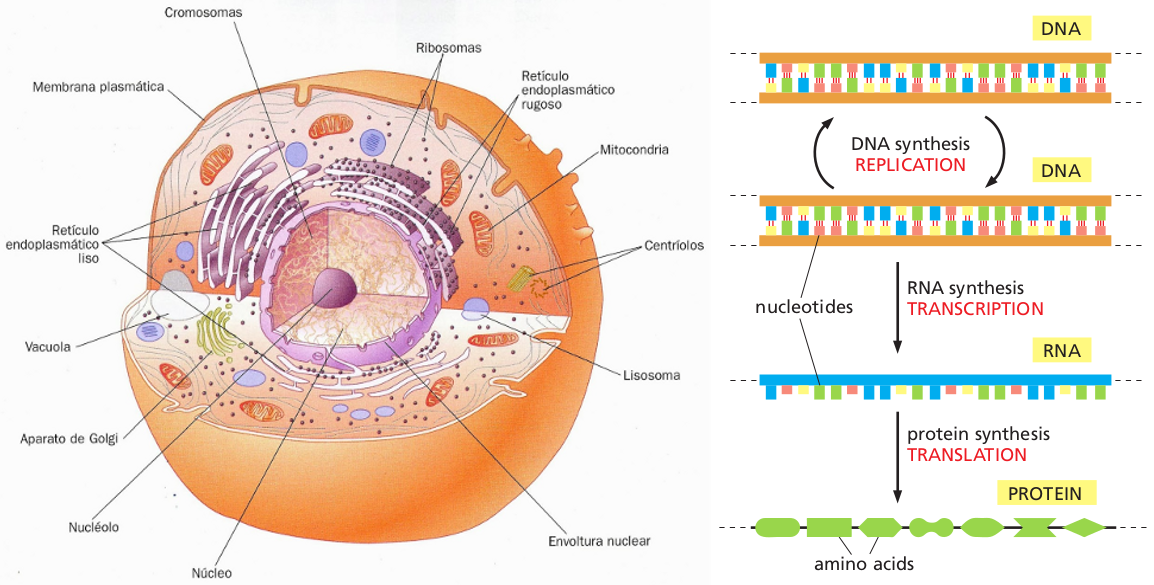
\includegraphics[width=1\textwidth]{celula_y_adn}
\end{columns}
\end{frame}

\subsubsection*{Cambios transcripcionales}
\begin{frame}\frametitle{Cambios transcripcionales en respuesta a estrés abiótico en \textit{A. thaliana}} 
	\begin{columns}[T]
		\column{0.5\textwidth}
			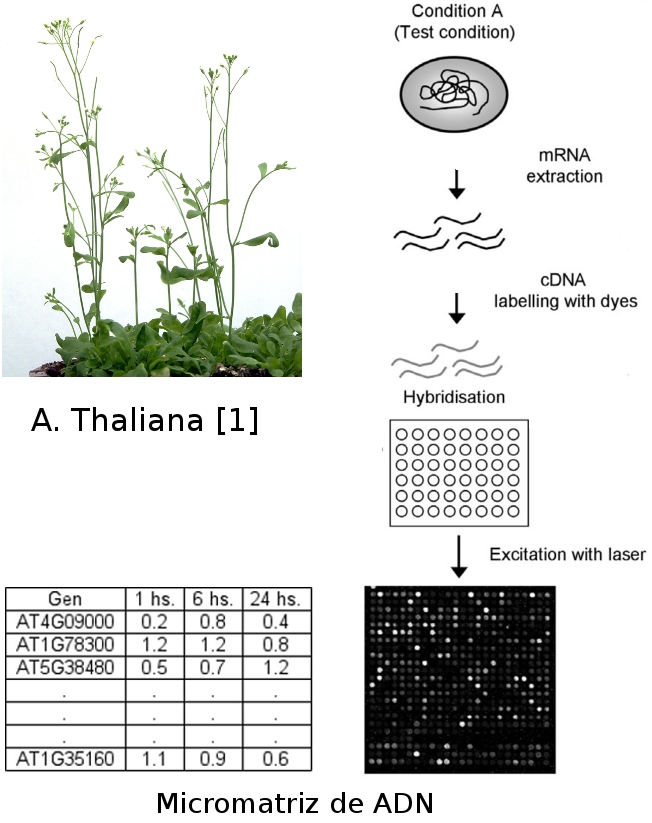
\includegraphics[width=1\textwidth]{micromatriz_y_arabidopsis}\\
			\tiny
			[1] arabidopsis.org: AtGenExpress.
		\column{0.5\textwidth}
			\Large 
			Datos de estrés abiótico:
			\medskip
			\Fontvi
			\begin{itemize}
				\item \textbf{10 tratamientos + control}: frío, calor, osmótico, salinidad, sequía, genotoxicidad, oxidación, UV, herida, recuperación.
				\item $\approx 22000$ genes.
				\item $\approx 6000$ genes se \textbf{movieron} en algún tratamiento.
				\item \textbf{Entre 4 y 8 mediciones} temporales por gen y por tratamiento.
			\end{itemize}			
			\centering	
			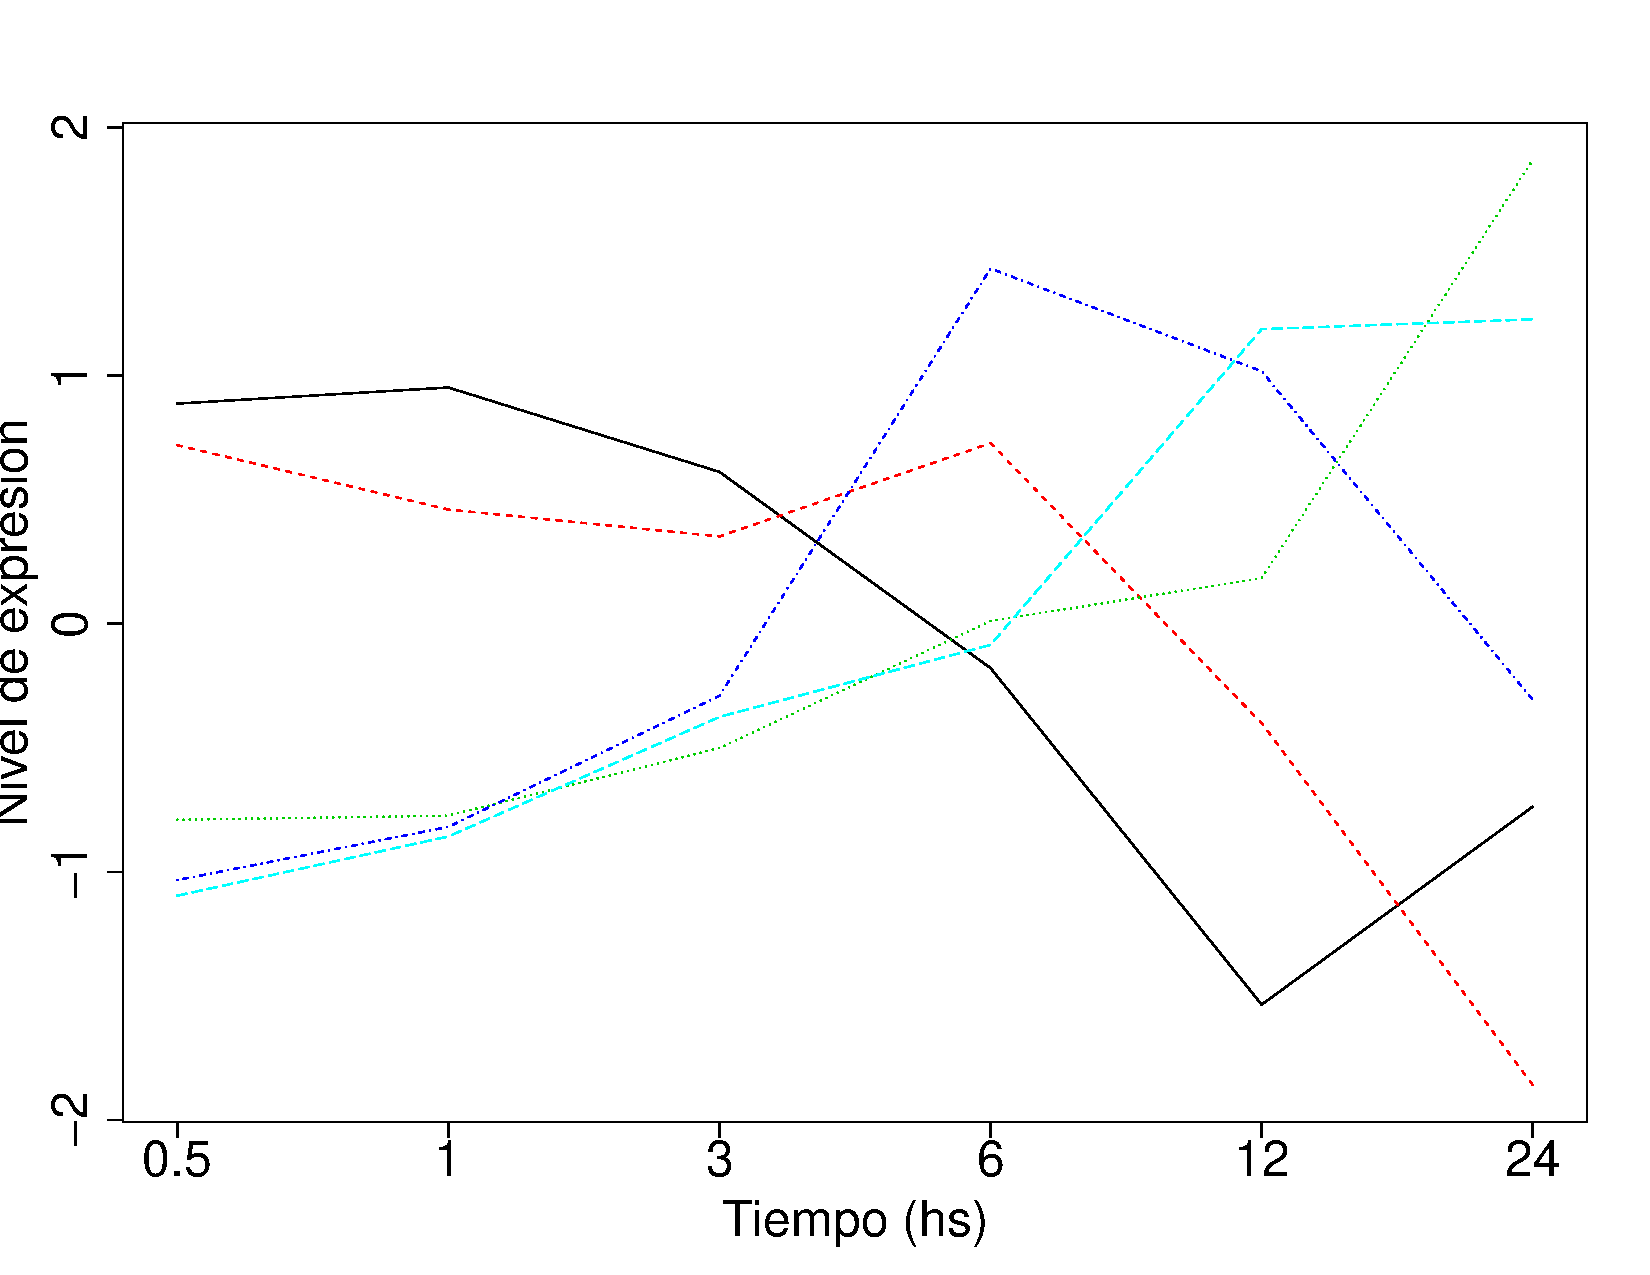
\includegraphics[width=0.95\textwidth]{perfiles_sin_agrupar.pdf}			
	\end{columns}
\end{frame}

\subsection{Detección de correlaciones}
\begin{frame}\frametitle{Detección de correlaciones} 
Queremos inferir estrategias del organismo frente a los tratamientos.\\\bigskip
Lo vamos a hacer usando \textbf{métodos de agrupamiento o ``clustering''} para encontrar relaciones y estructura en esta gran cantidad de datos.\medskip
\begin{columns}[T]
	\column{0.5\textwidth}
\begin{itemize}
\item Son métodos no supervisados.
\item Consisten en agrupar elementos \textbf{``similares entre sí''}.
\item Permiten el \textbf{descubrimiento de patrones} en los datos.
\item Posibilitan obtener \textbf{conclusiones} sobre los datos.
\end{itemize}
\column{0.5\textwidth}
\centering
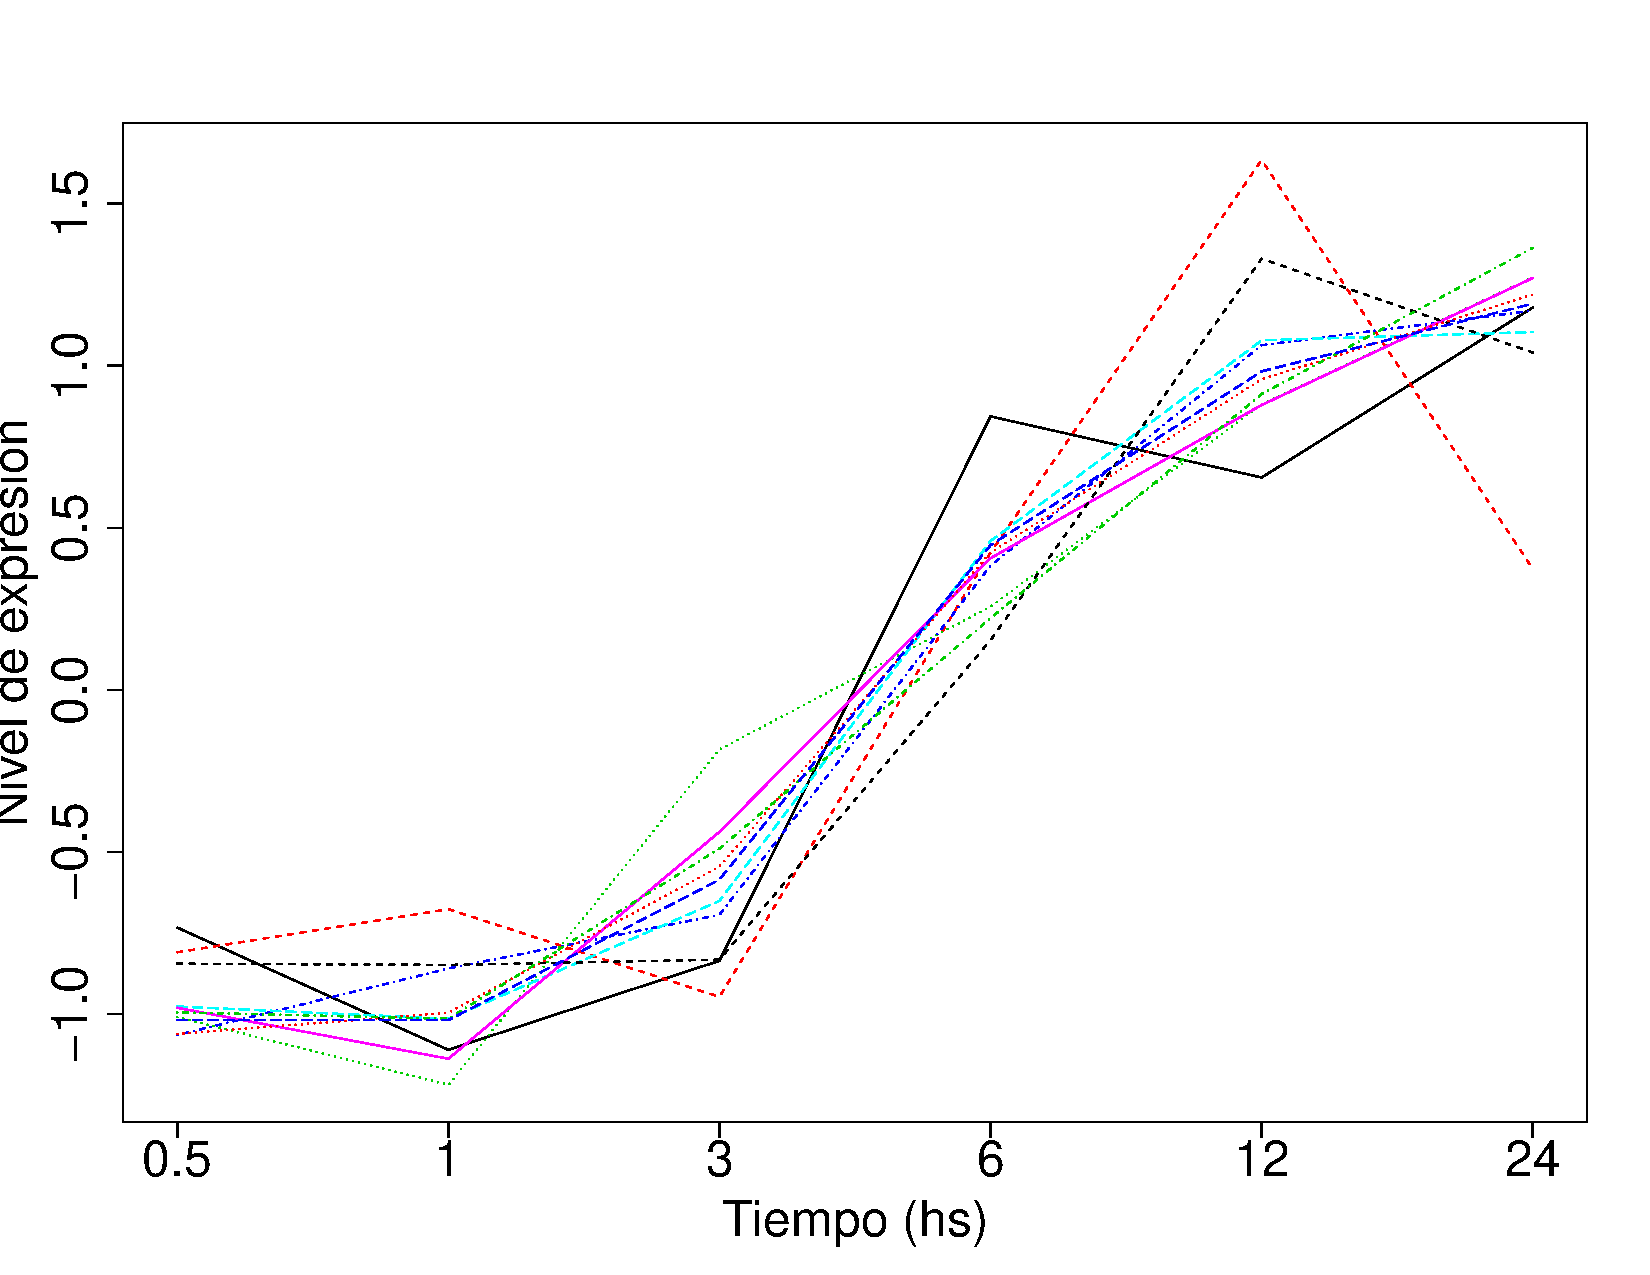
\includegraphics[width=1\textwidth]{perfiles_coregulados.pdf}
\end{columns}
\end{frame}

\section{Análisis de relevamientos transcripcionales}

\subsection{Medidas de similaridad y distancia}
\begin{frame} \frametitle{Usamos el coeficiente de correlación de Pearson} 
\begin{columns}
\column{\dimexpr\paperwidth-30pt}
\vspace{30pt}
\begin{columns}[T]
    \column{0.4\textwidth}
	\centering
	Distancia basada en el coeficiente de correlación de Pearson\\
	\Fontvi
	\begin{equation*}
		r(\vec{x}, \vec{y}) = \frac{\frac{1}{n-1}\sum\limits_{i=1}^n(x_i-\bar{x})(y_i-\bar{y})}{s_x s_y}
	\end{equation*}
	\begin{equation*}
		d_{ccp}(\vec{x}, \vec{y}) = 1-r(\vec{x}, \vec{y})
	\end{equation*}
    \column{0.6\textwidth}
	\centering	
	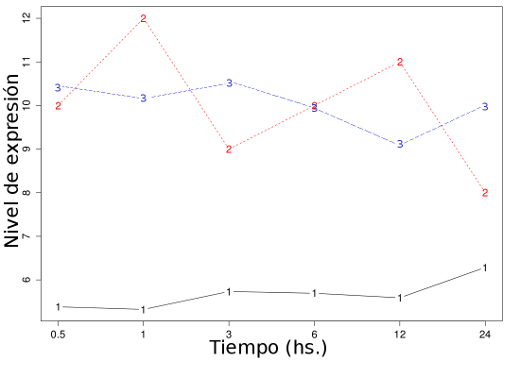
\includegraphics[width=0.9\textwidth]{perfiles_ejemplo_metricas.png}\\
\end{columns}
\end{columns}
\end{frame}

\subsection{Métodos de agrupamiento utilizados}
\begin{frame}\frametitle{Métodos de agrupamiento} 
\begin{columns}[T]
\small
\column{0.4\textwidth}
Método k-means\\
\begin{itemize}
	\item Busca estructuras compactas.
	\item Muy rápida ejecución. 
	\item La cantidad k de grupos debe ser fijada a priori.  
	\item Existen figuras de mérito para decidir el k óptimo.
\end{itemize}
\bigskip
\bigskip
Método corte de árbol dinámico\\
\begin{itemize}
	\item Agrupamiento jerárquico.
	\item Representación mediante \textbf{dendrograma}.
	\item Ajuste por \textit{deepsplit} (usamos DS1 y DS4).
\end{itemize}			
	\column{0.6\textwidth}
    \centering
    \vspace{-10pt}
    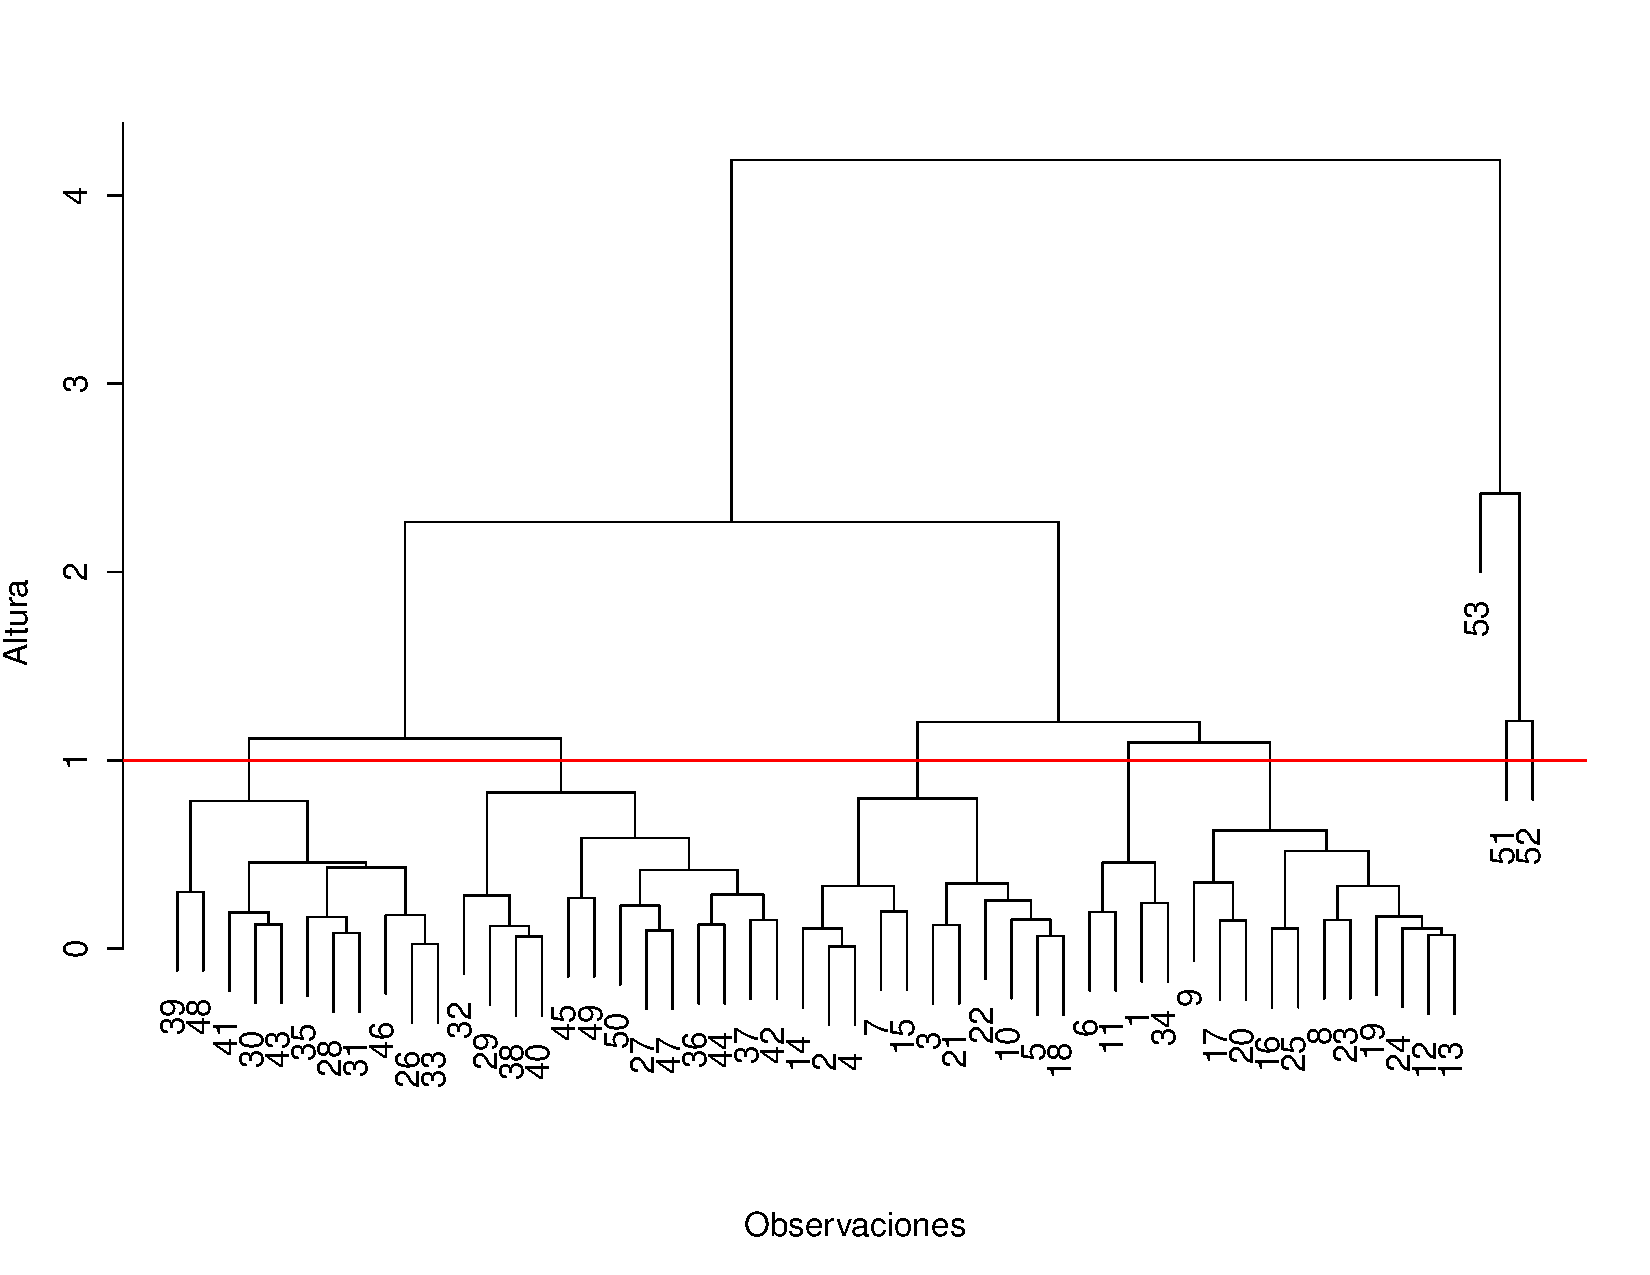
\includegraphics[width=1.1\textwidth, height=1\textheight]{dendrograma_muestra.pdf}
\end{columns}
\end{frame}

\begin{frame}\frametitle{Ejemplo de agrupamientos} 
\begin{figure}
\centering
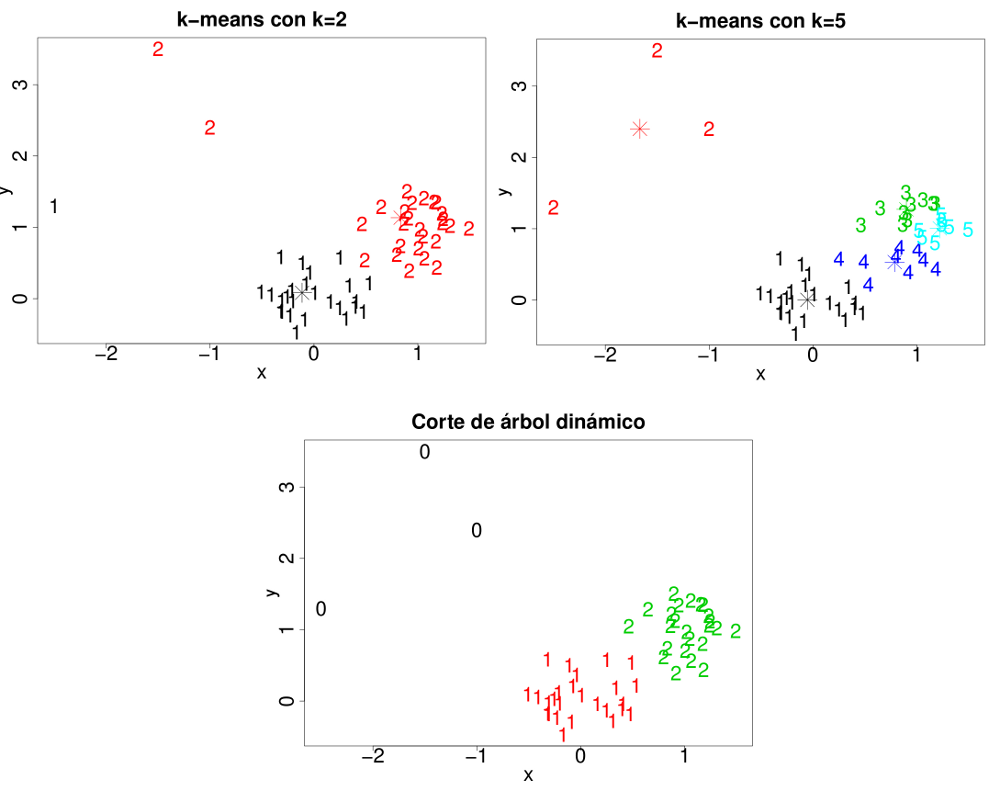
\includegraphics[width=0.85\textwidth]{ejemplo_agrupaciones.png}
\end{figure}
\end{frame}

\subsection{Caracterización de particiones}
\begin{frame}\frametitle{Grupos con k-means} 
\begin{columns}
\column{\dimexpr\paperwidth-20pt}
\centering
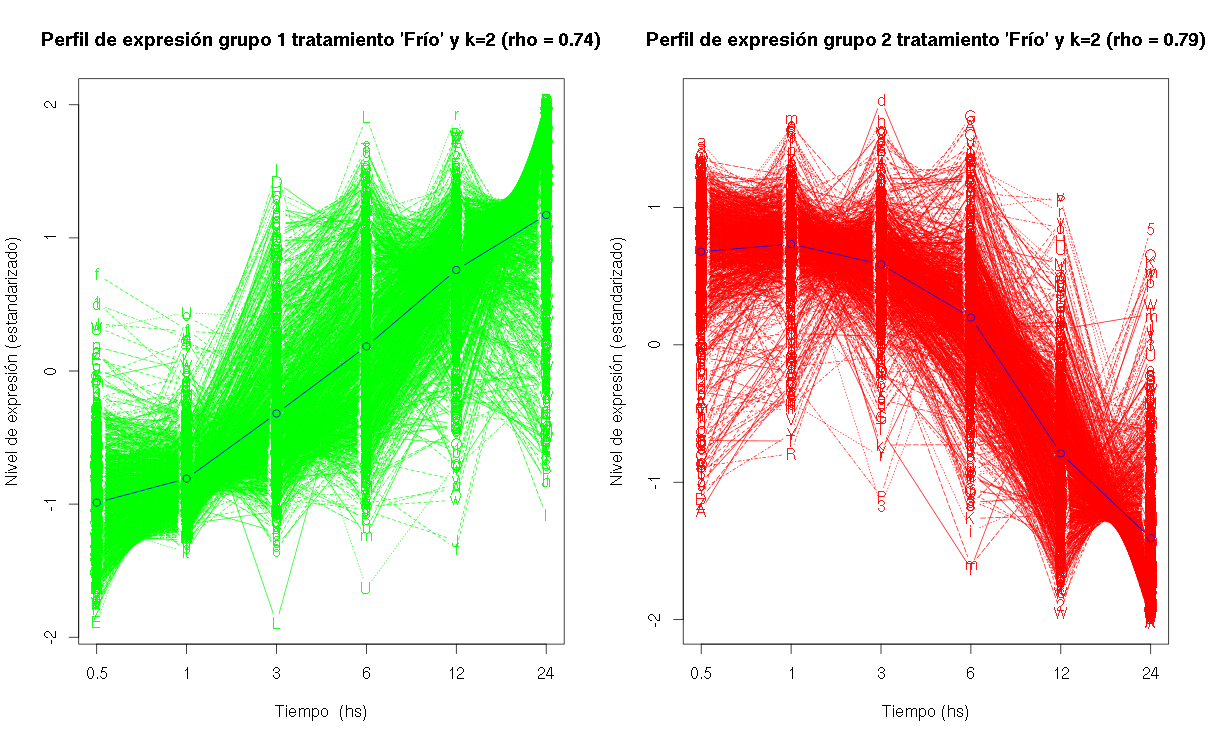
\includegraphics[width=1\textwidth]{perfiles_k_means}	
\end{columns}
\end{frame}

\begin{frame}\frametitle{Grupos con corte de árbol dinámico} 
\centering
A modo de ejemplo, los nueve perfiles más grandes de una partición de tratamiento ``Frío'' y DS1.\\
\begin{figure}
\centering
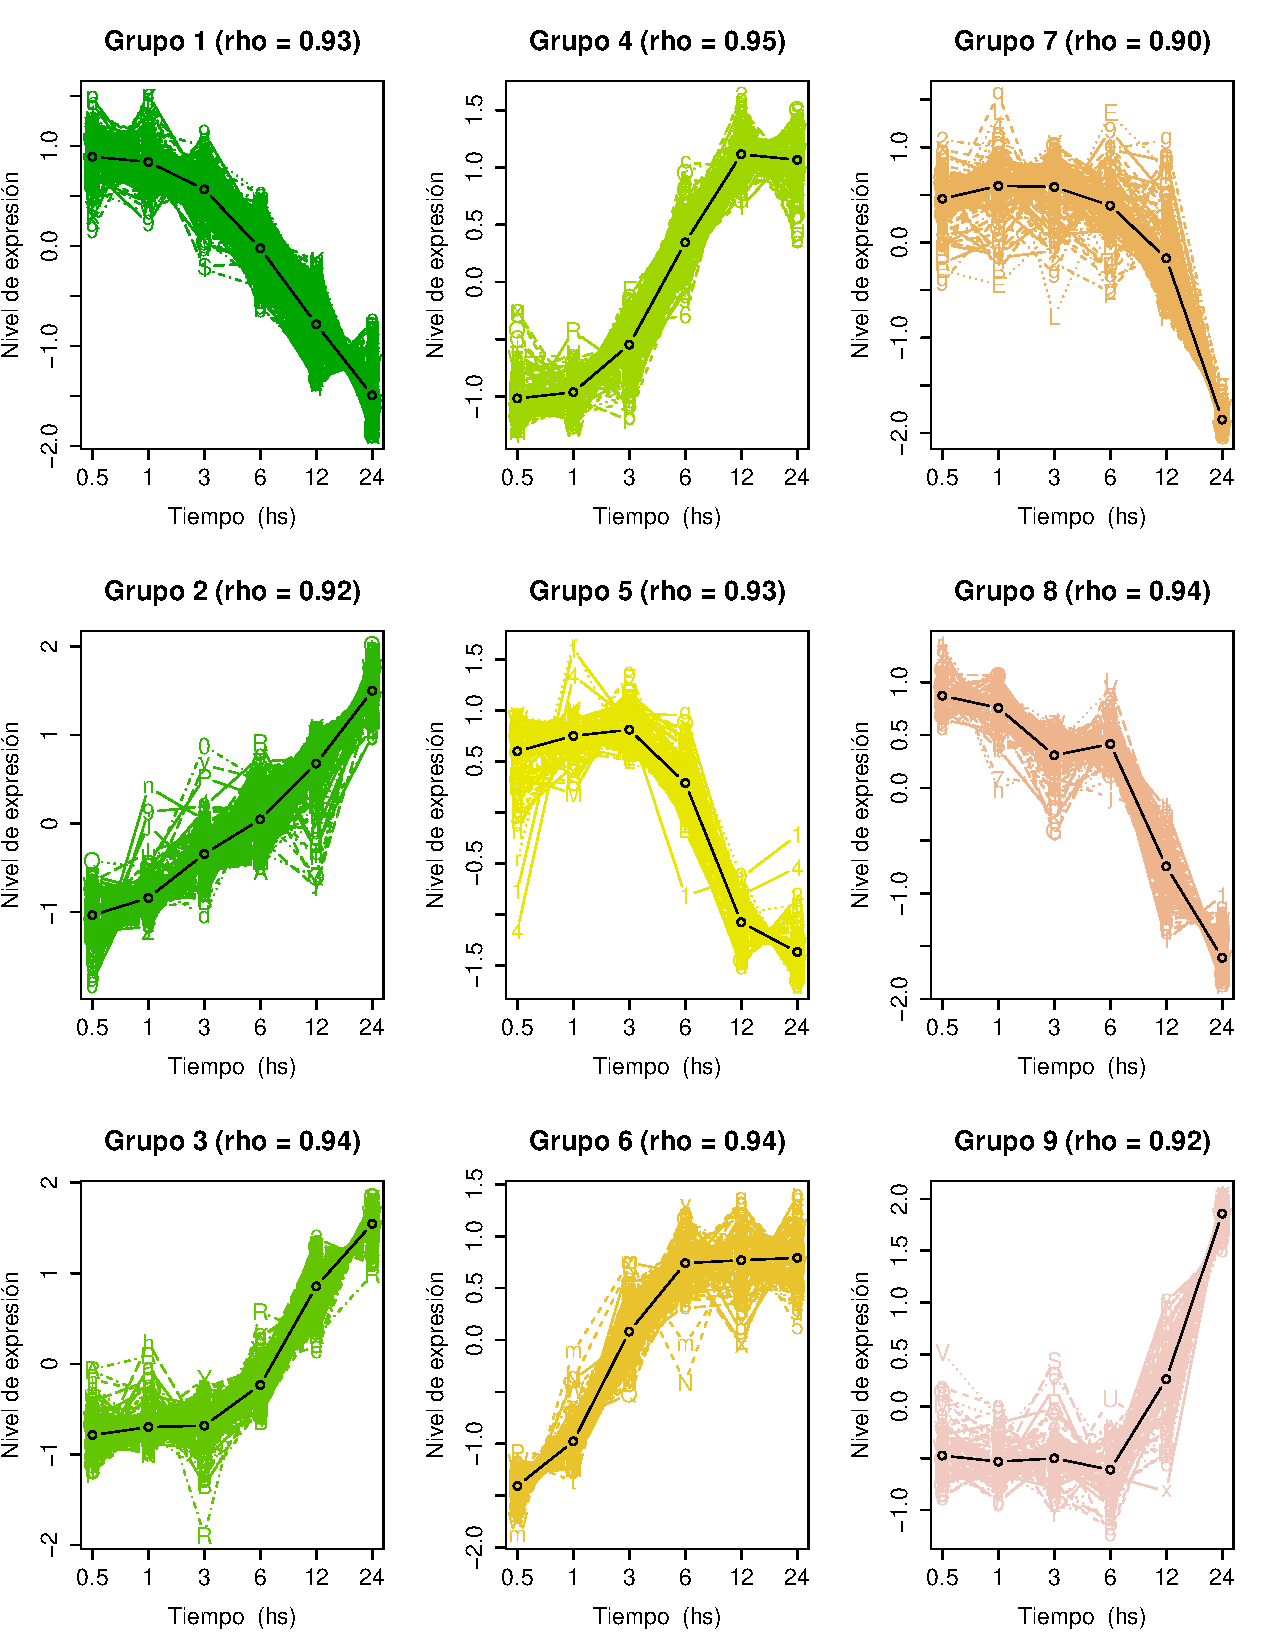
\includegraphics[width=0.8\textwidth, height=0.8\textheight]{perfiles_ds_1.pdf}	
\end{figure}
\end{frame}

%\begin{frame}\frametitle{Caracterización de particiones corte de árbol dinámico} 
%\centering
%Correlación media por tamaño de grupo
%\begin{columns}[T]
%\column{0.5\textwidth}
%	\centering
%	DS1 (particiones más gruesas)
%	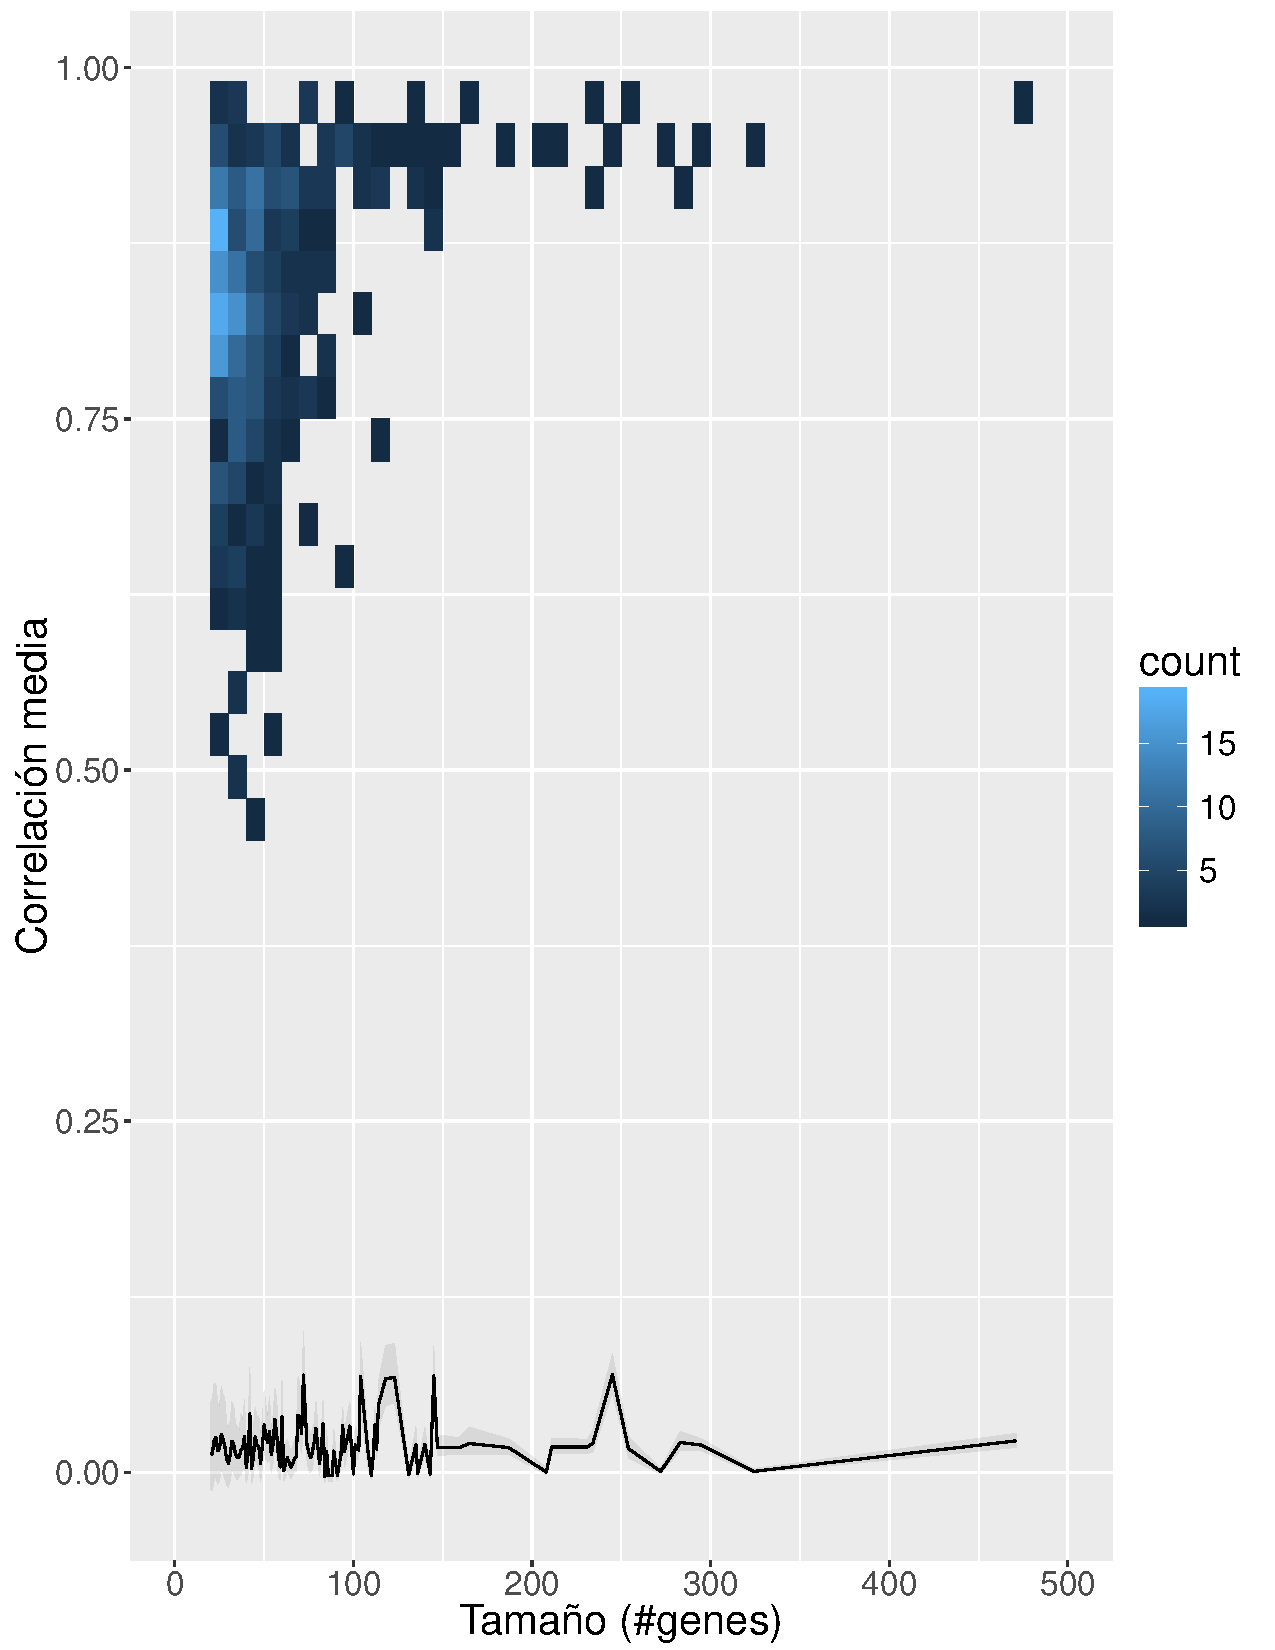
\includegraphics[width=0.9\textwidth]{correlacion_media_por_tamano_ds_1.pdf}	
%\column{0.5\textwidth}
%	\centering
%	DS4 (particiones más finas)
%	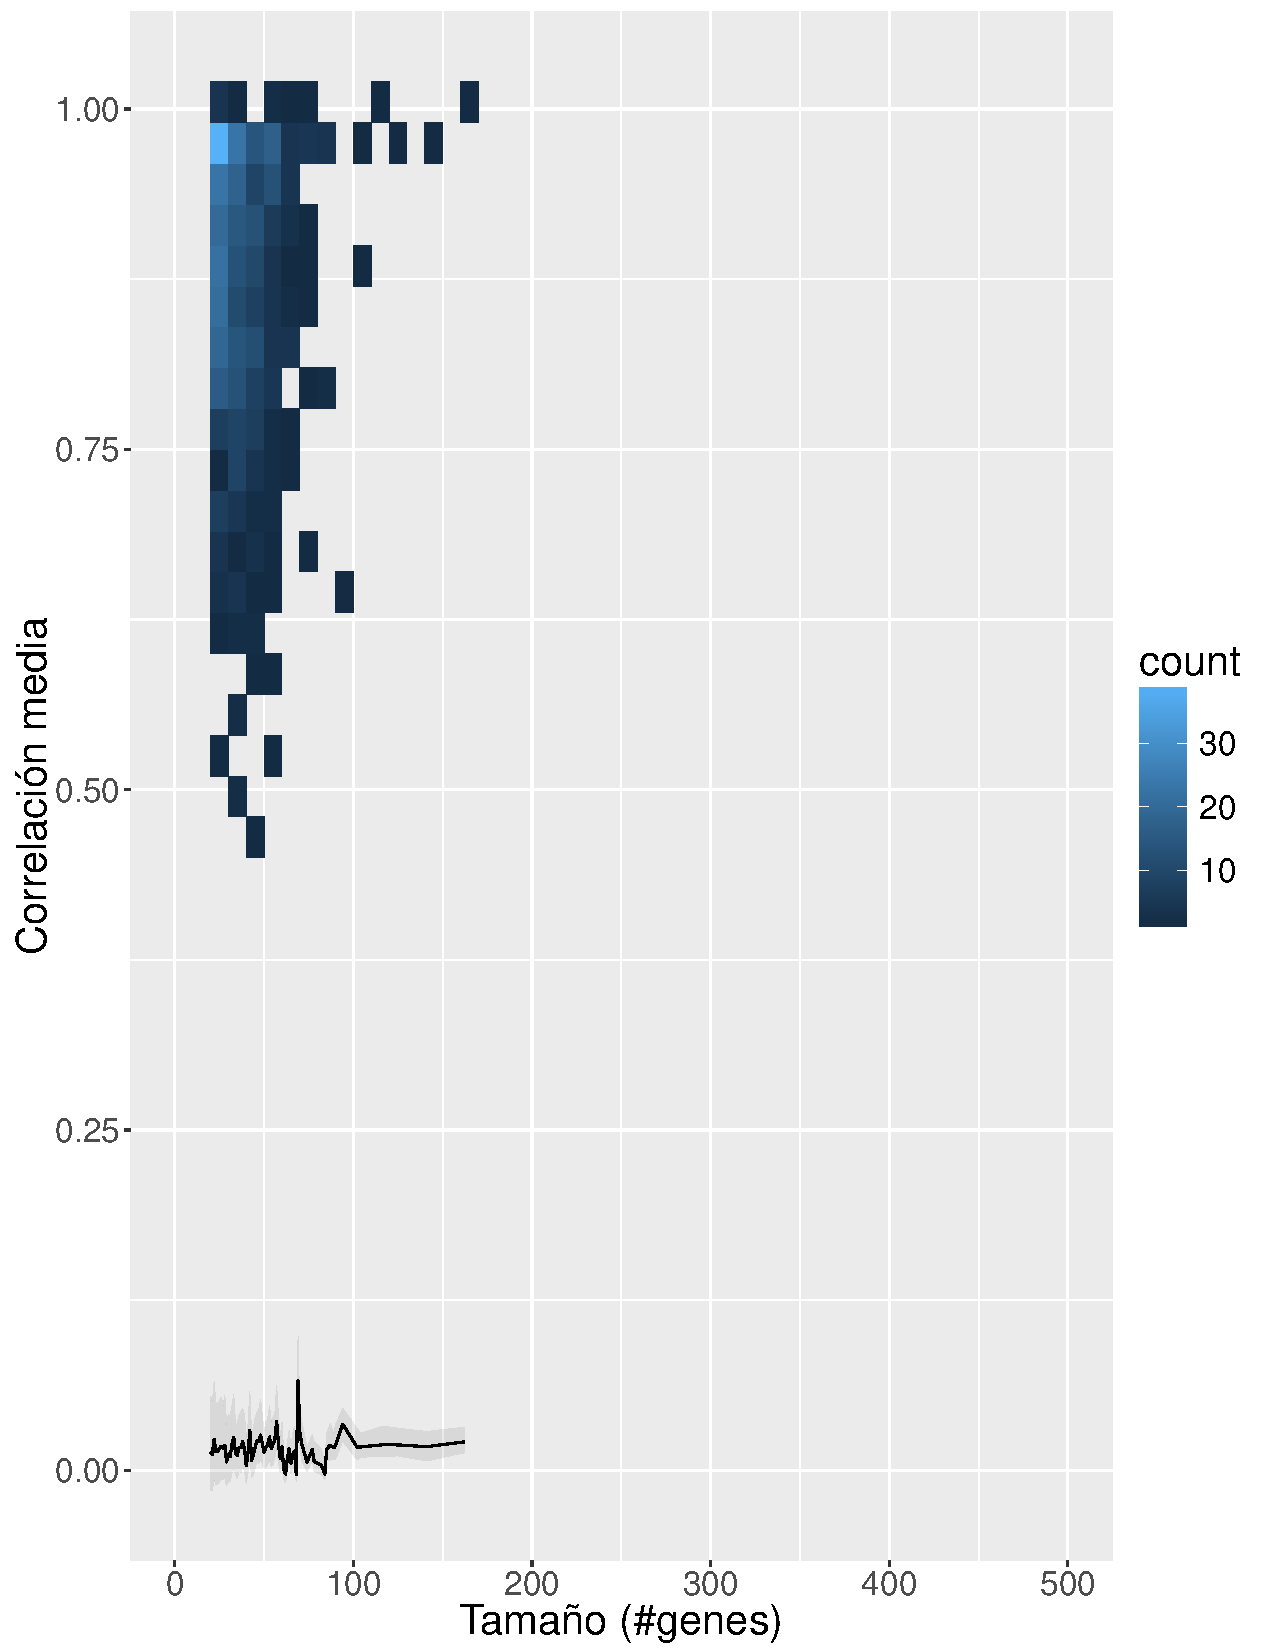
\includegraphics[width=0.9\textwidth]{correlacion_media_por_tamano_ds_4.pdf}	
%\end{columns}
%\end{frame}

%\begin{frame}\frametitle{Caracterización de granularidad de las particiones halladas} 
%\centering
%Fracción de grupos en una partición más fina dentro de grupos de una partición más gruesa (tratamiento ``Frío'')
%\begin{figure}
%    \centering
%	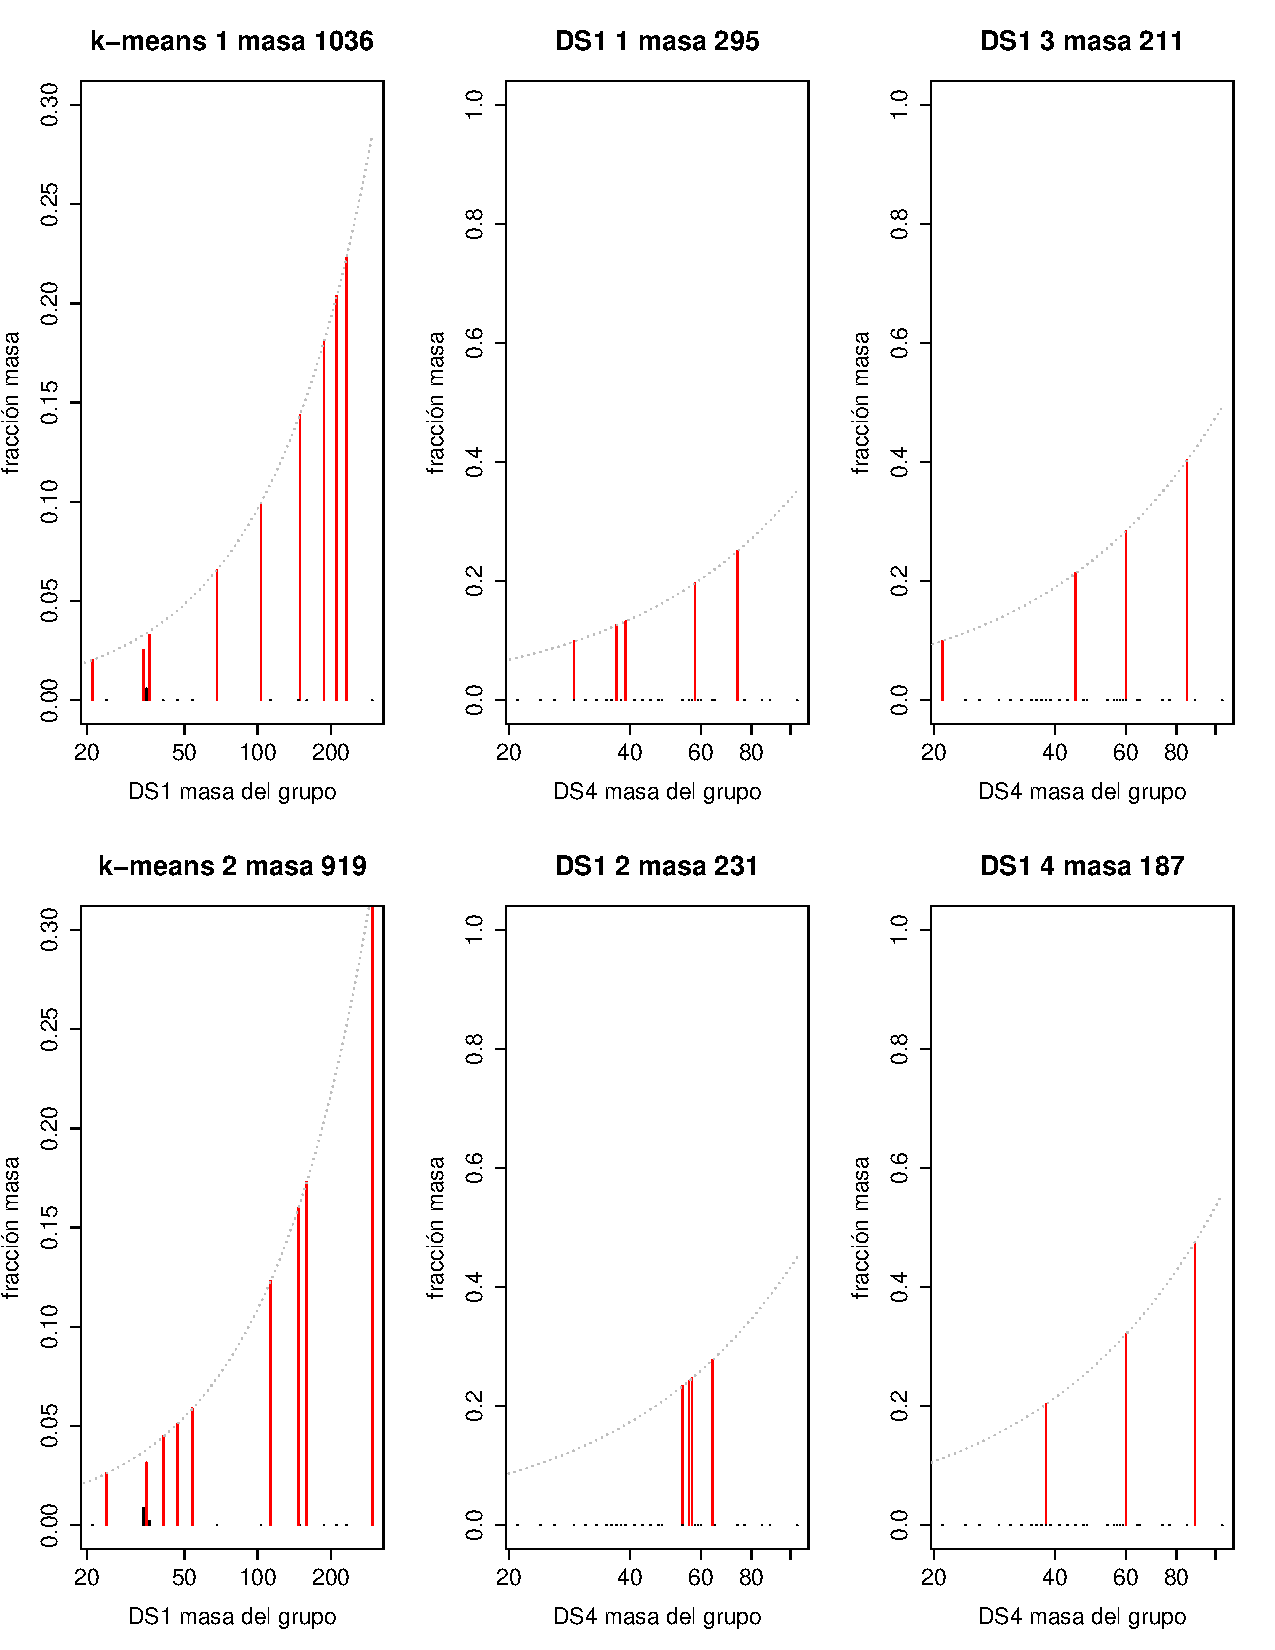
\includegraphics[height=1.6\textheight]{fraccion_de_km_en_ds1_en_ds4.pdf}	
%\end{figure}
%\end{frame}

\begin{frame}\frametitle{El problema de la escala} 
Granularidad y resolución de los métodos
\bigskip
\begin{itemize}
\item Una partición $A$ es \textbf{más fina} que una partición $B$ si cada grupo de $A$ está contenido en un grupo de $B$.
\item Tenemos \textbf{tres formas de realizar particiones} de nuestros datos.
\item DS4 genera particiones más finas que DS1 y este a su vez que k-means.
\item Tenemos distintas maneras de encontrar estructura en nuestros datos y las \textbf{distintas heterogeneidades aparecerán a distintas escalas}.
\end{itemize}
\bigskip
Vamos a ver si existe una \textbf{escala óptima en un sentido biológico} a la que trabajar con éste conjunto de datos y para eso vamos a utilizar un espacio de conocimiento biológico.\\
\hfill
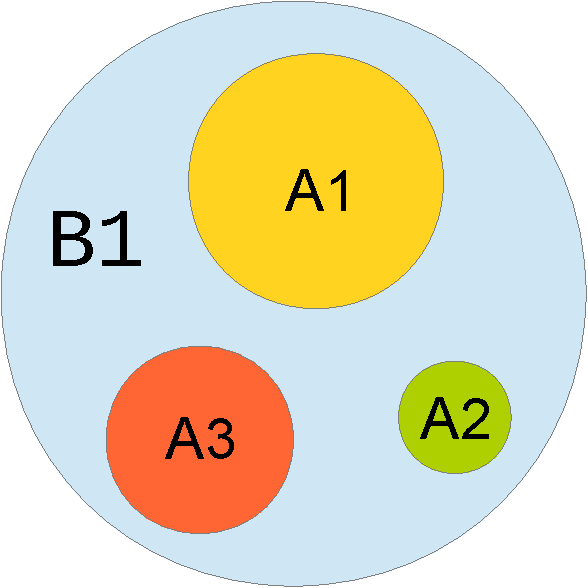
\includegraphics[width=0.2\textwidth]{granularidad.pdf}	
\end{frame}

\section{Congruencia biológica}

\subsection{Ontología génica (GO)}
\begin{frame}\frametitle{Ontología génica (GO)}
\begin{columns}[T]
	\column{0.5\textwidth}
	\begin{itemize}
		\item Provee un vocabulario controlado de términos.
		\item Permite comparar y clasificar entidades biológicas.
		\item Tres ontologías: procesos biológicos (BP), componentes celulares (CC) y funciones moleculares (MF).
		\item Estructura de grafo acíclico dirigido (DAG).
		\item Cada nodo representa un término que describe alguna función.
		\item Los nodos se unen entre si por medio de relaciones ``es un'' o ``es parte de''.
	\end{itemize}
	\column{0.5\textwidth}
	\centering
	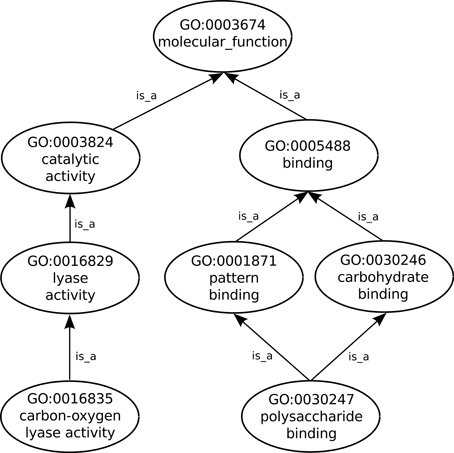
\includegraphics[width=1\textwidth]{ejemplo_de_go.jpg}	
	
	\medskip
	\Fontvi
	Un gen descrito por un término está ``anotado'' en ese término.	
\end{columns}
\end{frame}

\subsection{Cuantificando la congruencia biológica}
\begin{frame}\frametitle{Observables} 
\centering
Buscamos cuantificar la congruencia biológica de las particiones halladas
\bigskip
\begin{columns}[T]
\column{0.45\textwidth}
Densidad de interacción:\\
\bigskip
\begin{equation}
ID(GO_j) = \frac{NE(GO_j)}{N(GO_j)}
\end{equation}\\
\bigskip
Con $NE(GO_j)$ la cantidad de pares de genes anotados en $GO_j$ que se encuentran juntos en un mismo grupo transcripcional $C_x$ y $N(GO_j)$ la cantidad de pares de genes anotados en $GO_j$.
\column{0.55\textwidth}
Indice de homogeneidad biológica:\\
\bigskip
\begin{equation*}
BHI_j = \frac{1}{n_j(n_j-1)}\sum\limits_{x\neq y\in D_j}I(C(x)=C(y))
\end{equation*}\\
\medskip	
Con $n_j$ la cantidad de genes anotados en el grupo $D_j$.\\
La función indicadora $I(C(x)=C(y))$ toma el valor $1$ si hay al menos una clase en donde ambos genes estén anotados, y $0$ en caso contrario.
\end{columns}
\end{frame}

\begin{frame}\frametitle{Densidad de interacción} 
\begin{columns}[T]
	\column{0.3\textwidth}
	\Fontvi
	\begin{enumerate}
	\item Términos mas específicos presentan mayor ID en una relación decreciente.
	\item DS1 presenta mayor congruencia biológica que DS4. Indicio acerca de la escala apropiada.
	\item Ambos presentan mayor congruencia biológica que el control nulo.
	\item Los agrupamientos inducidos por otra información presentan mayor congruencia que los inducidos por expresión.
	\end{enumerate}
	\column{0.7\textwidth}
	\begin{figure}
	    	\centering
		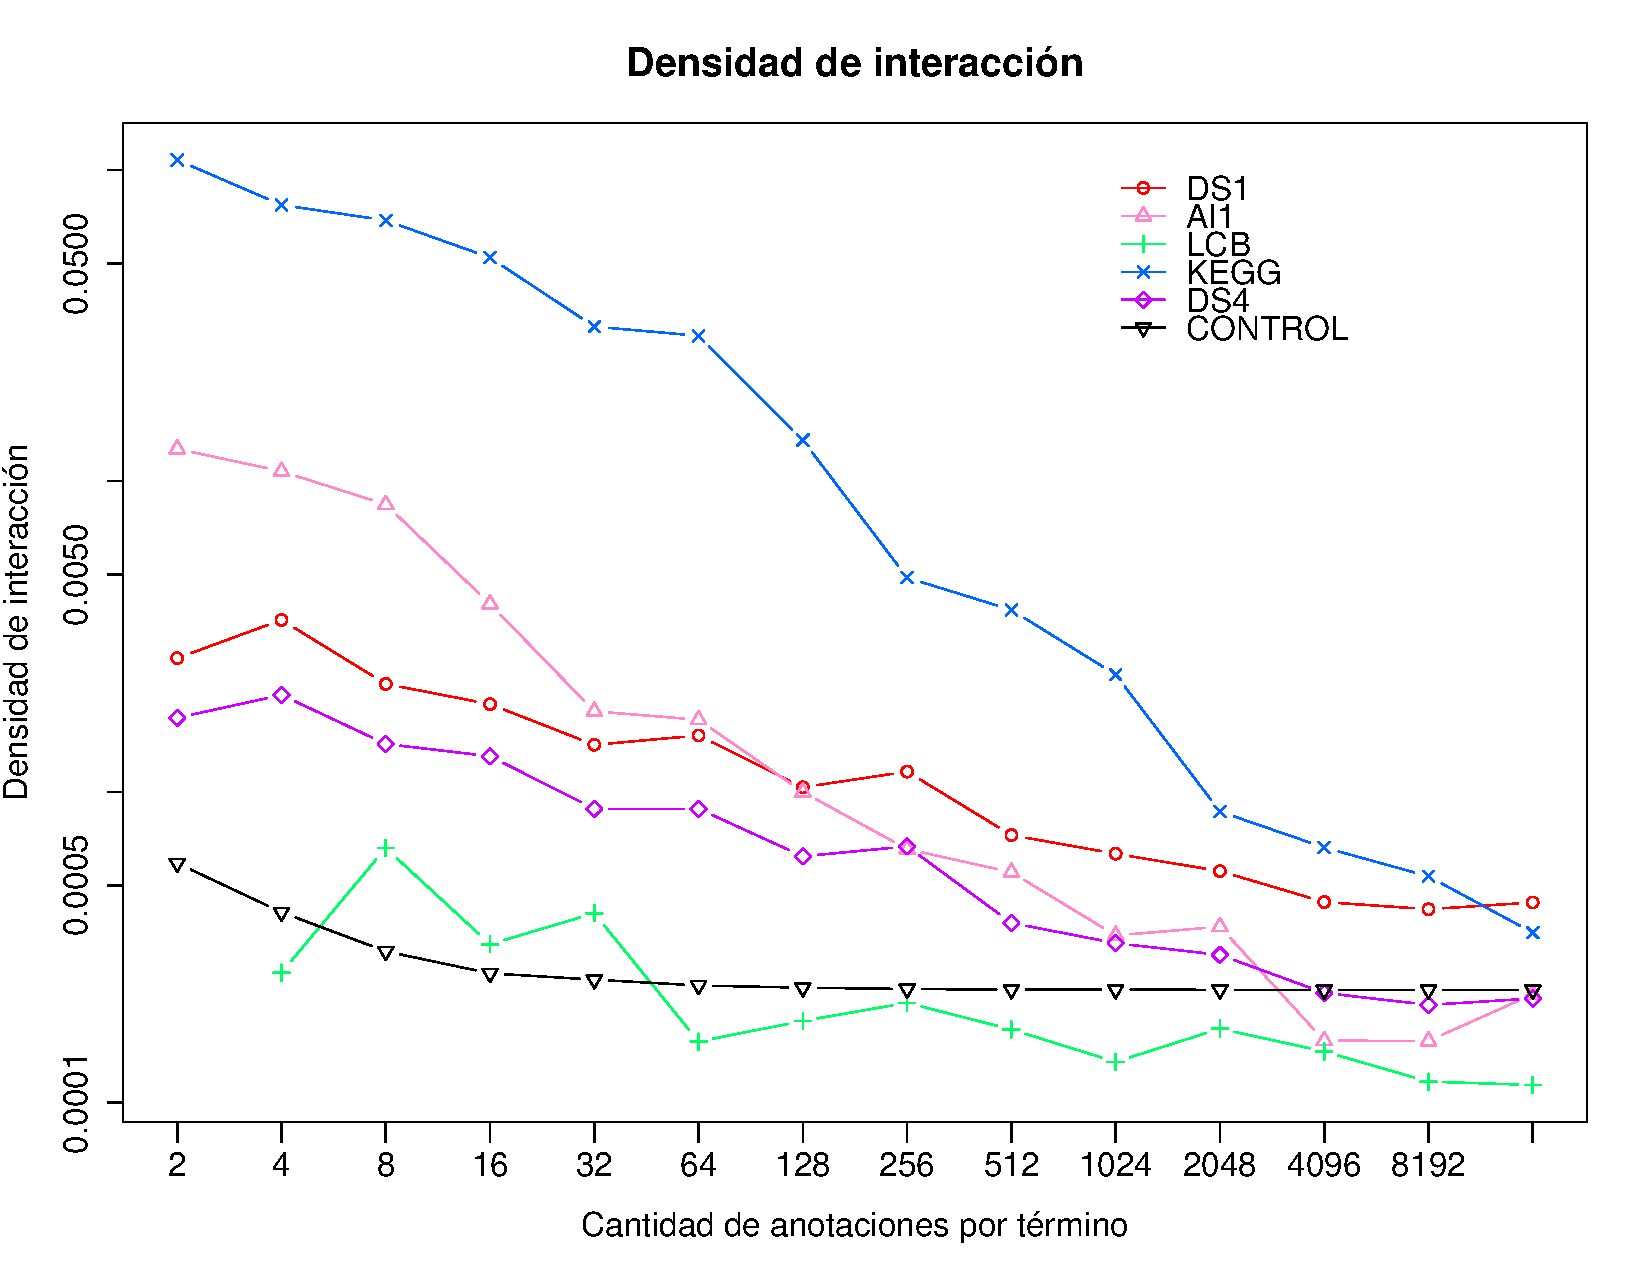
\includegraphics[width=1\textwidth]{interacting_densities_bpb.pdf}
	\end{figure}
\end{columns}
\end{frame}

\begin{frame}\frametitle{Indice de homogeneidad biológica} 
\begin{figure}
    	\centering
	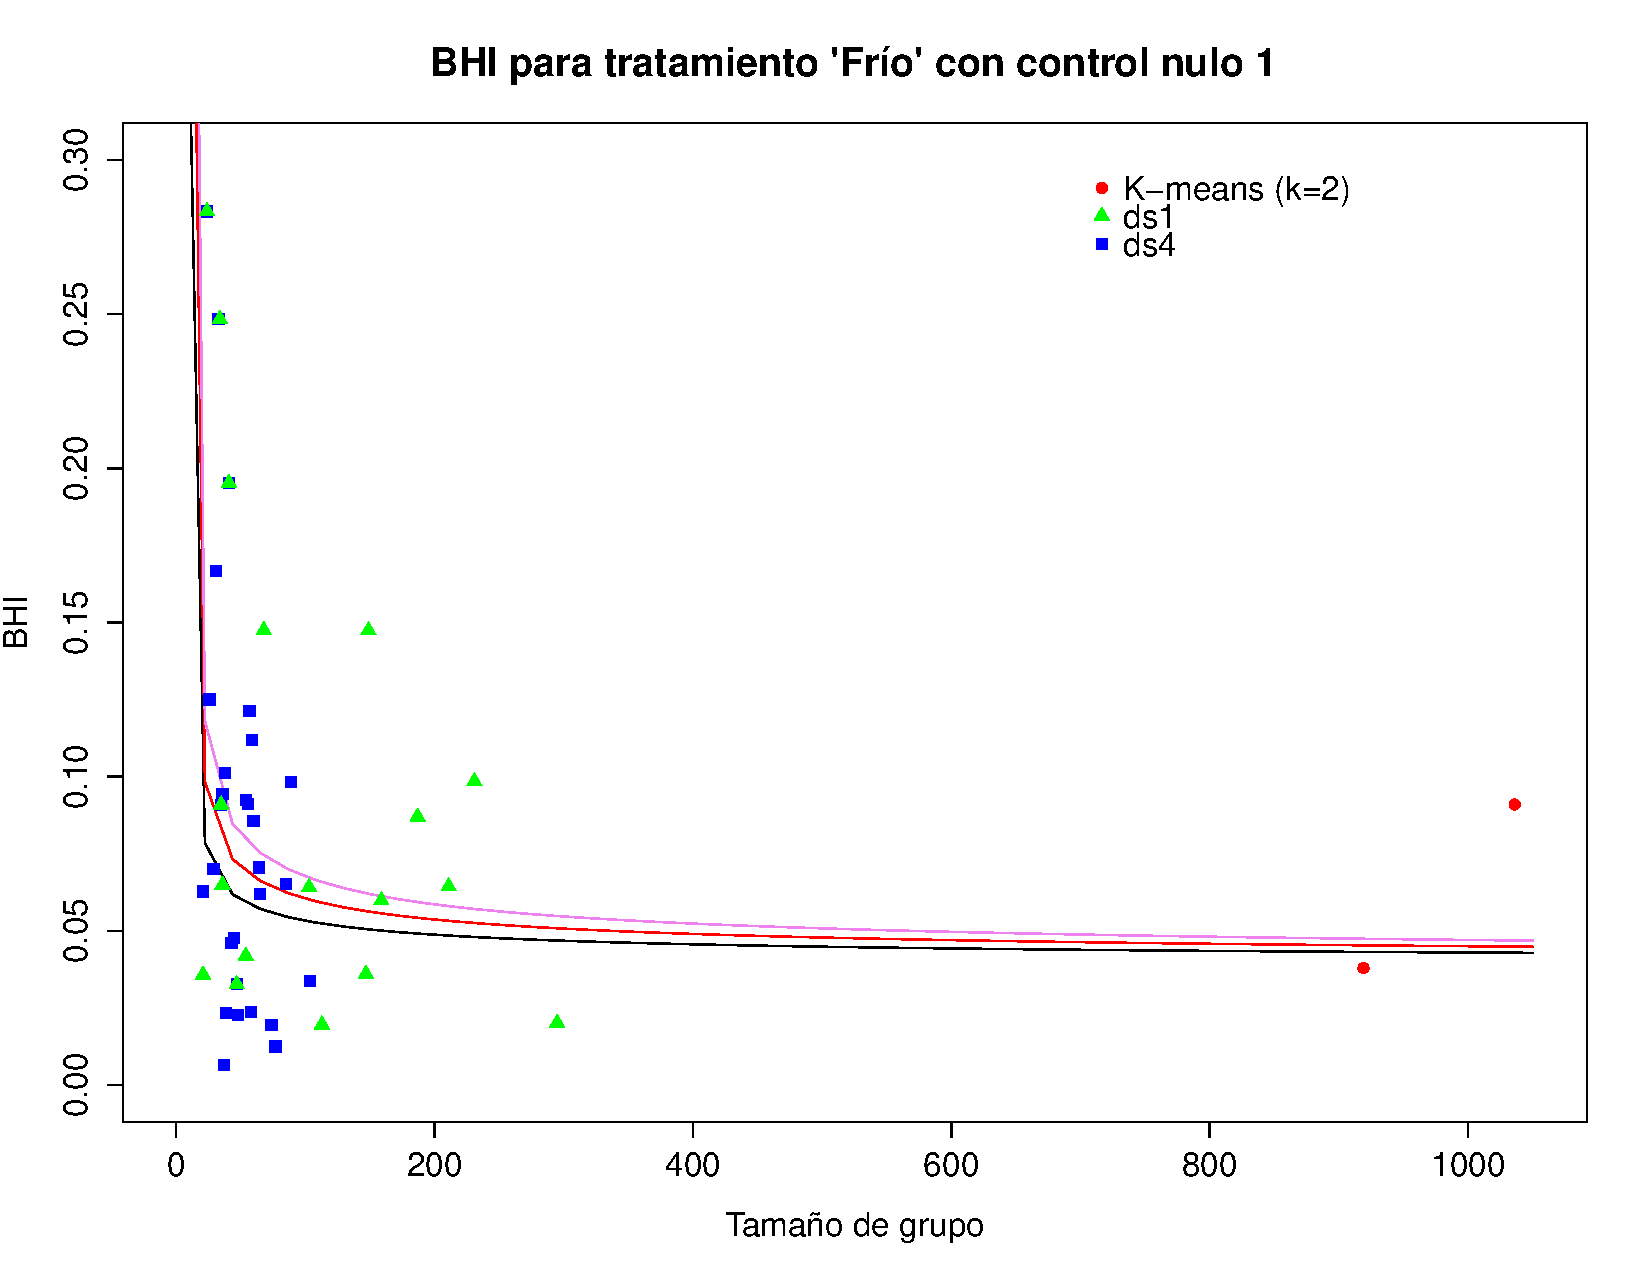
\includegraphics[width=0.78\textwidth]{bhi_km_ds1_ds4_control1.pdf}
\end{figure}
\Fontvi
\centering
Grupos altamente coherentes pero de baja calidad de BHI. No tienen soporte biológico.
\end{frame}

\section{Coherencia entre métricas}

\subsection{Métrica en GO}
\begin{frame}\frametitle{Similaridad entre genes en GO}
\centering
Podemos definir similaridades entre genes en el espacio GO\\
\bigskip
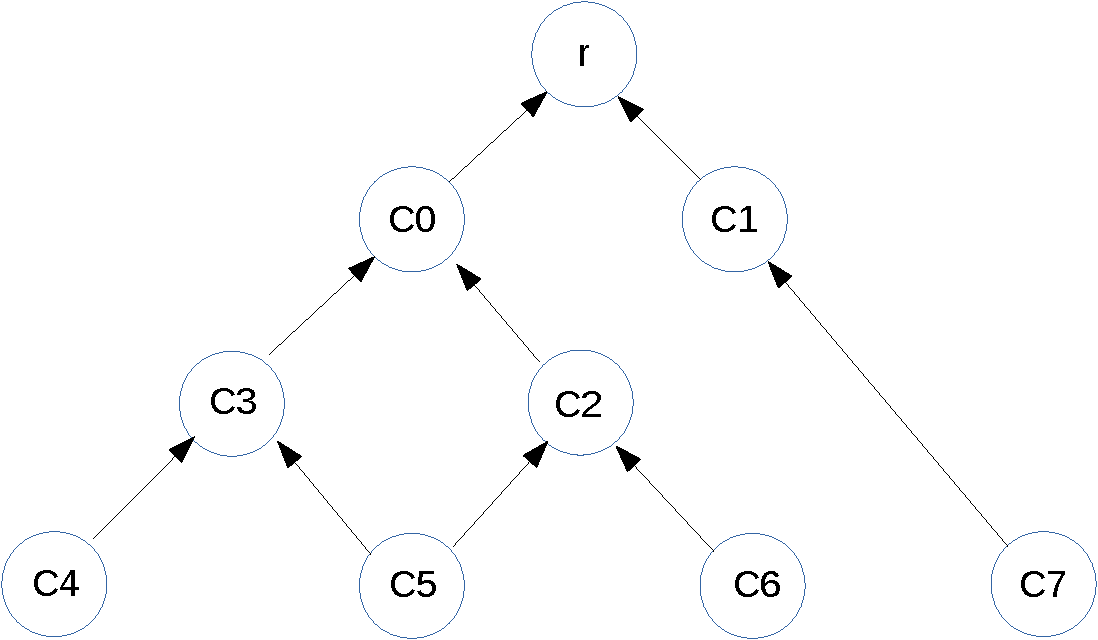
\includegraphics[width=0.5\textwidth]{dag.pdf}
\\\bigskip
Utilizando la similaridad entre términos:
\begin{equation}
	Sim_{res}(c_i, c_j) = \max\limits_{c \in S(c_i, c_j)}(-log_2[P(c)]) = IC(MICA[c_i, c_j])
\end{equation}
\end{frame}

\subsection{KTA global}
\begin{frame}\frametitle{KTA global} 
La noción de similaridad de a pares en cada espacio está dada en términos de una función $k$ llamada kernel tal que
\begin{equation}
	K = K_{ij} = k(x_i, x_j)
\end{equation}
\bigskip
El KTA de un kernel $k_1$ con respecto a un kernel $k_2$ del conjunto $C$ cuantifica la similaridad entre dos espacios y se define como:
\begin{equation}
	\hat{A}(C, k_1, k_2) = \frac{\langle K_1, K_2 \rangle _F}{\sqrt{\langle K_1, K_1 \rangle _F \langle K_2, K_2 \rangle _F}}
\end{equation}
con $\langle K_1, K_2 \rangle _F = \sum_{i,j=1}^m K_1(x_i, x_j)K_2(x_i, x_j)$ es el producto interno de Frobenius.\\
Intuitivamente, si $\langle K_1, K_2 \rangle$ es grande, ambos kernels son coherentes.
\end{frame}

\begin{frame}\frametitle{KTA global} 
\centering
KTA global entre expresión y ontología BP con control nulo
\begin{figure}
    	\centering
	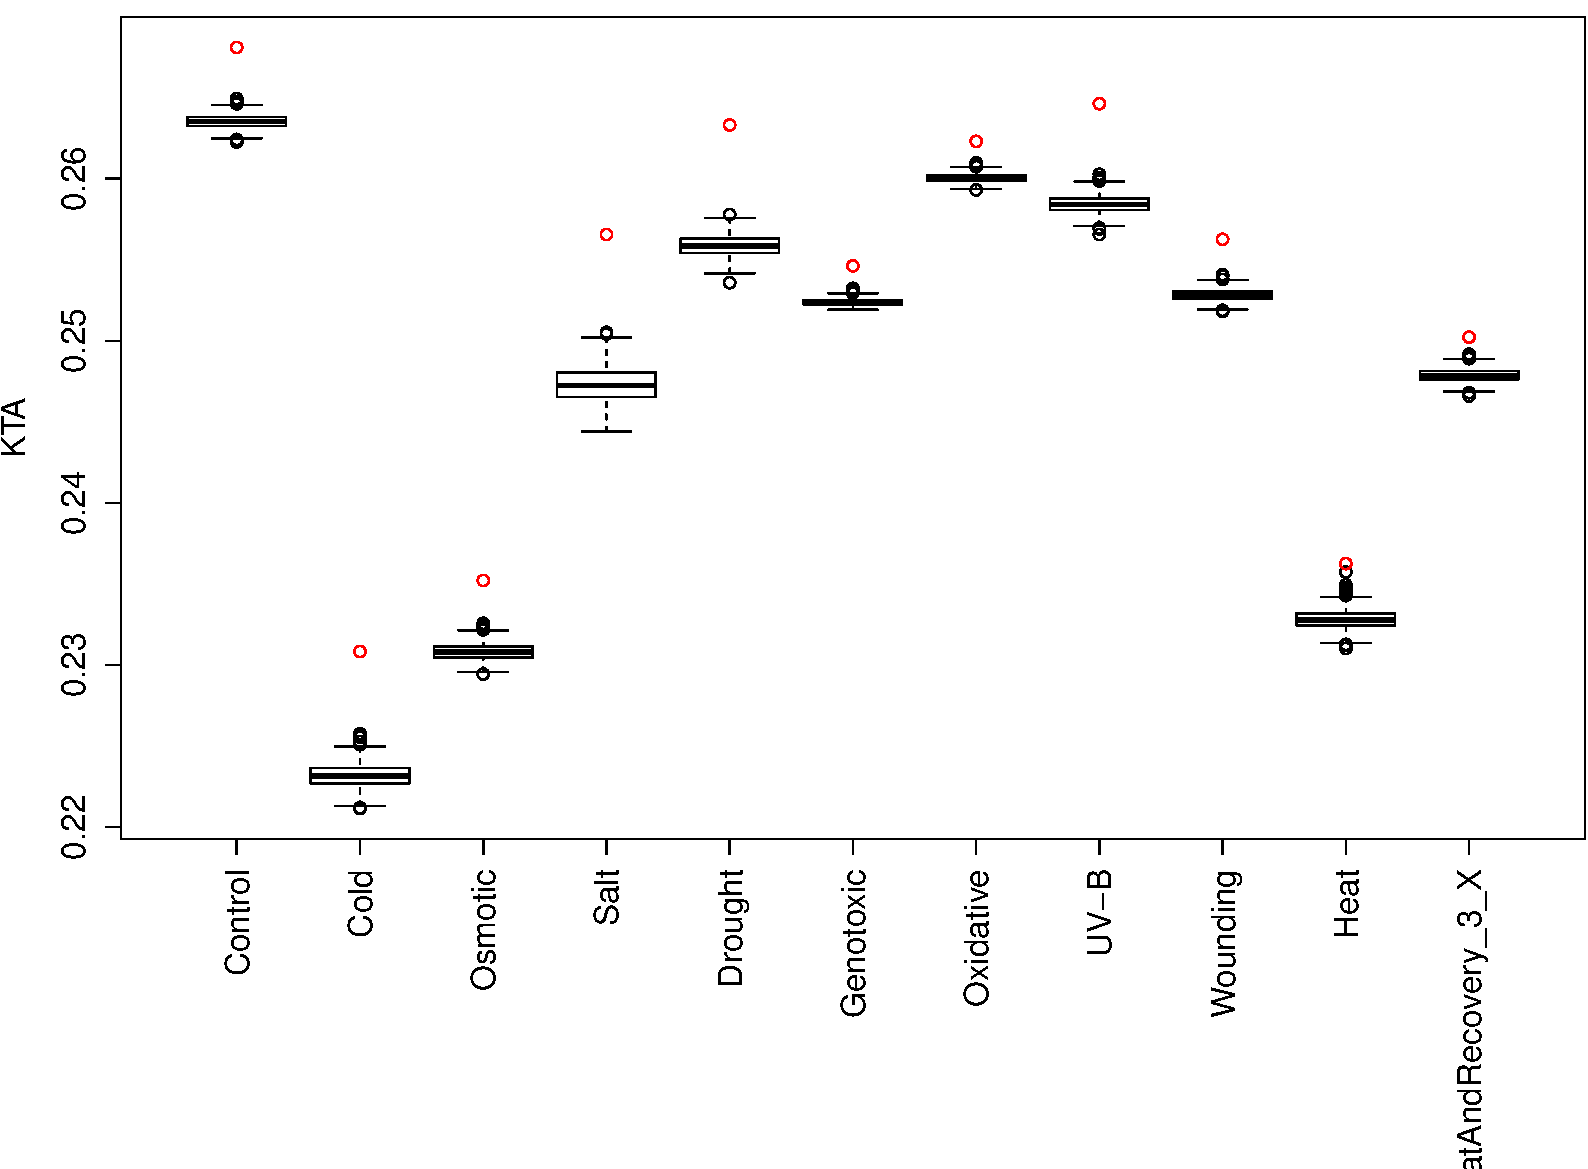
\includegraphics[width=0.8\textwidth]{kta_global_bpb.pdf}
\end{figure}
\centering
\end{frame}

\subsection{Modulación de heterogeneidades
transcripcionales con GO}
%\begin{frame}\frametitle{Red 30 primeros vecinos mutuos} 
%\bigskip
%\begin{columns}[T]
%	\column{0.5\textwidth}
%	\centering
%   Distribución de grado\\	
%  \bigskip
%    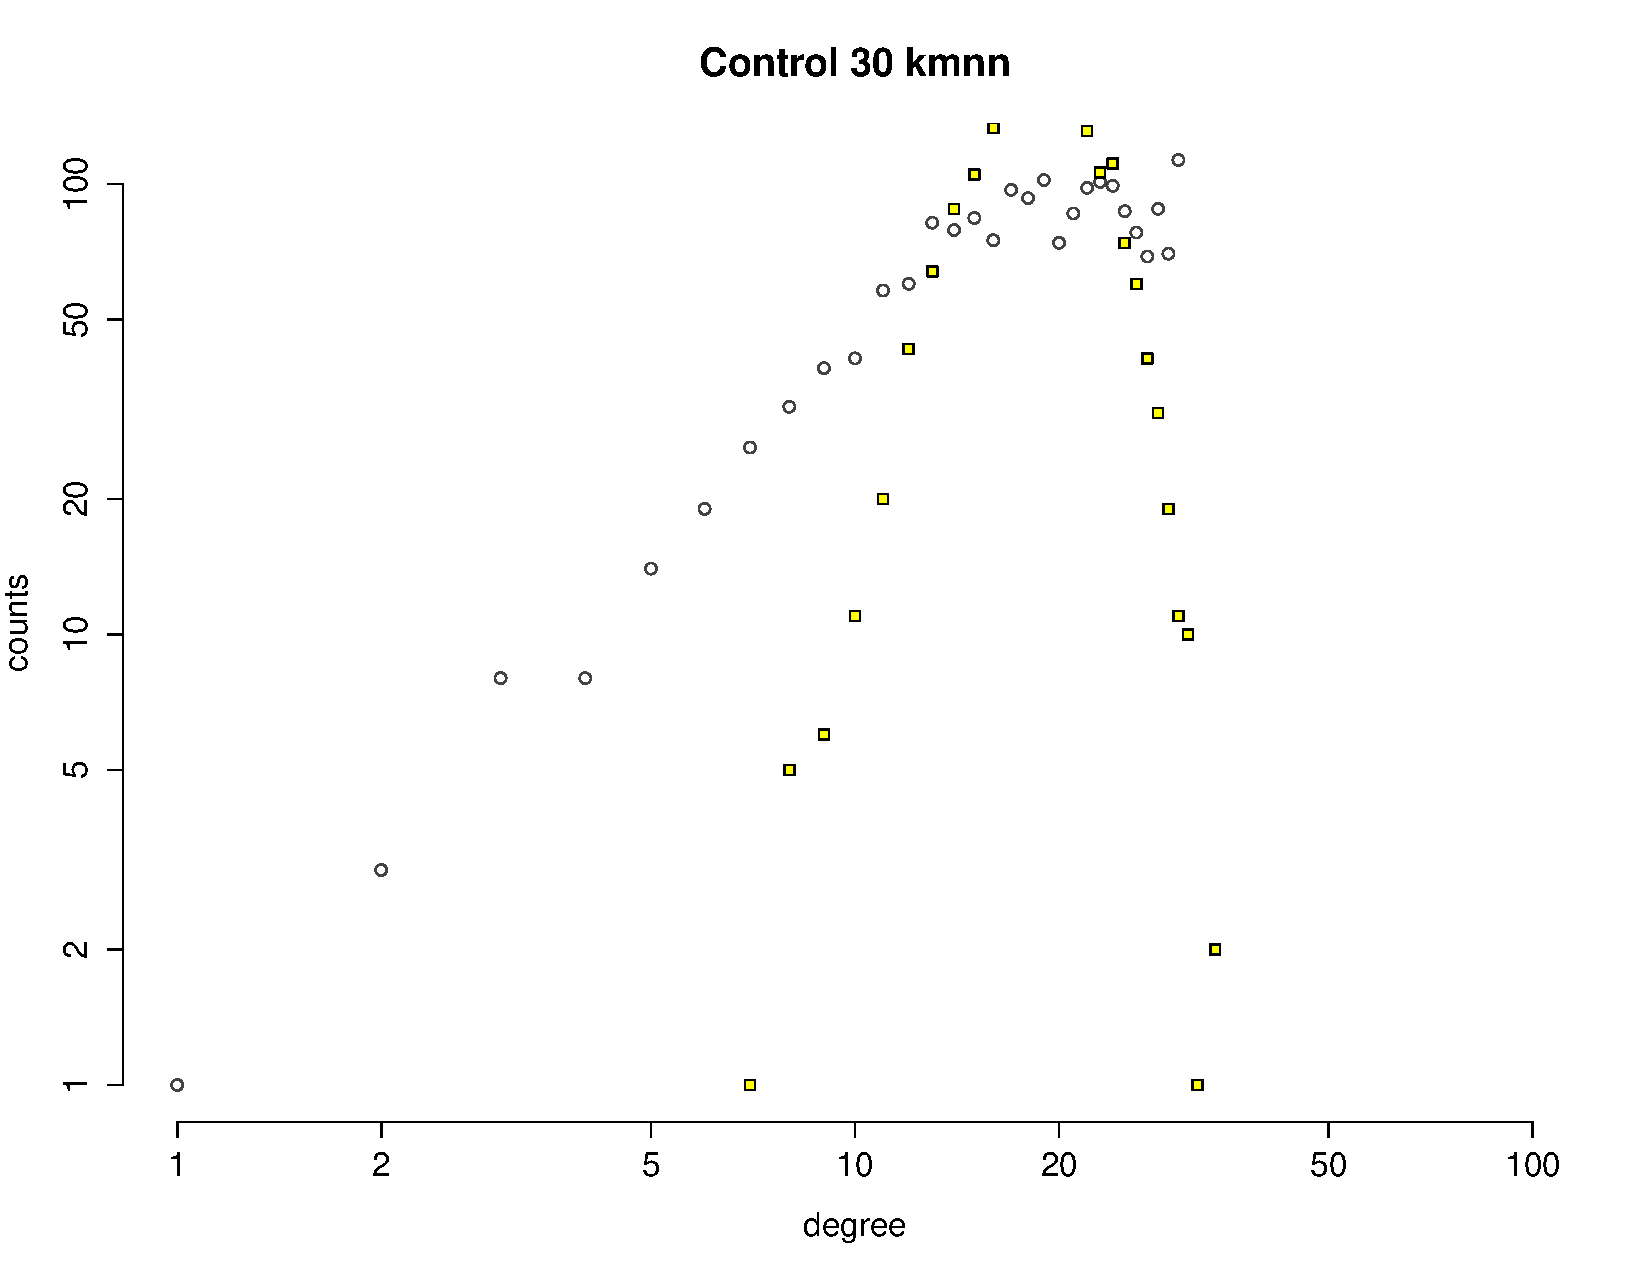
\includegraphics[width=1\textwidth]{erdos_renyi_vs_30kmnn.pdf}\\
%    Red y modelo nulo Erdös-Renyi
%    \column{0.5\textwidth}
%    \centering
%    Betweenness\\
%    \bigskip
%    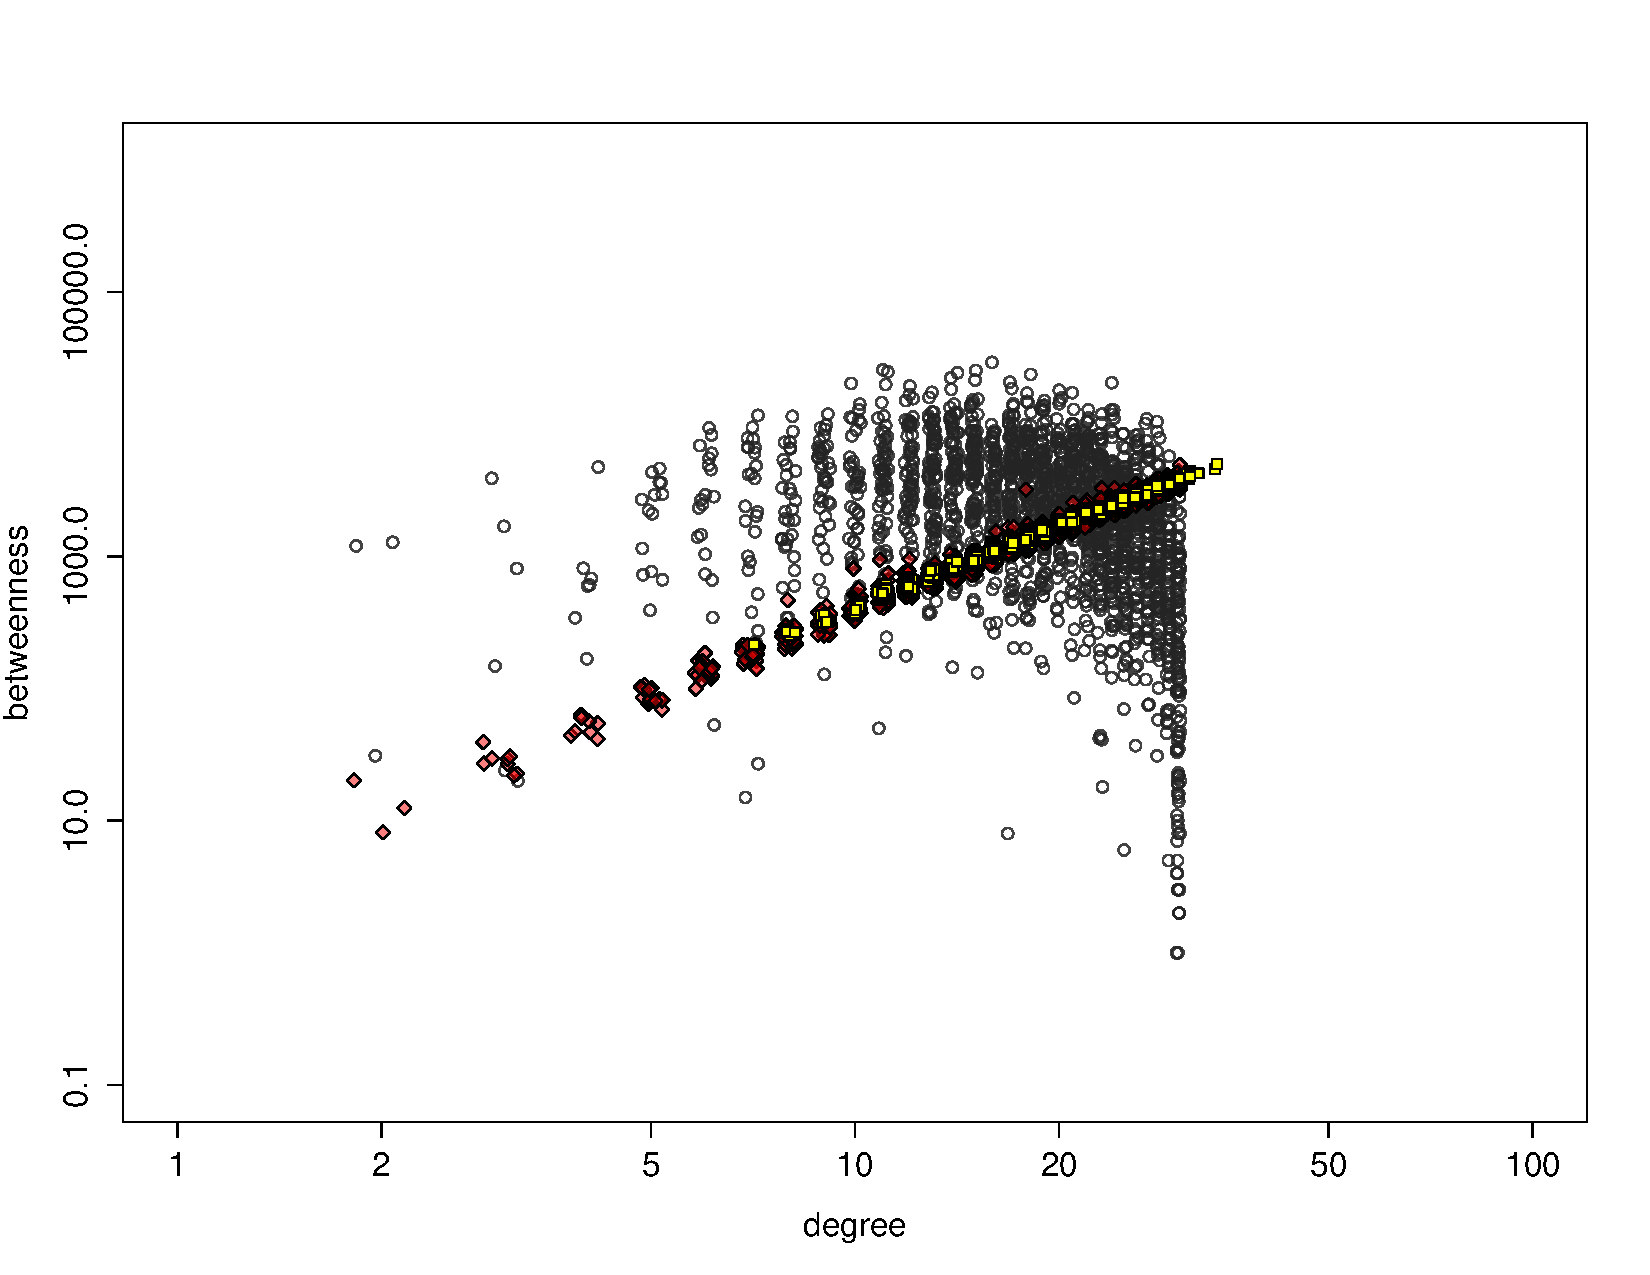
\includegraphics[width=1\textwidth]{betweenness_er_30_conf.pdf}\\
%    Red, modelo nulo Erdös-Renyi y modelo configuracional
%\end{columns}
%\end{frame}

\begin{frame}\frametitle{Red 30 primeros vecinos mutuos - vecindades locales} 
\centering
Queremos detectar zonas de alta coherencia.\\
\bigskip
\begin{columns}[T]
	\column{0.5\textwidth}
	 Generamos una red de 30 primeros vecinos mutuos y vamos a ver arista por arista, una localidad definida por los primeros vecinos:\\
	\begin{itemize}
	\item $n_x$ nodos.
	\item $n_y$ nodos anotados.
	\item $w_y$ distancia entre nodos $i$ y $j$ en GO.
	\item $w_{ny}$ similaridades promedio en una vecindad en GO.
	\item $w_{ny anotados}$ similaridades promedio en una vecindad en GO con nodos anotados.	
	\item $ktal_{anotados}$ KTA en la vecindad de los nodos anotados.		
	\end{itemize}
    \column{0.5\textwidth}
    \centering
    \bigskip
    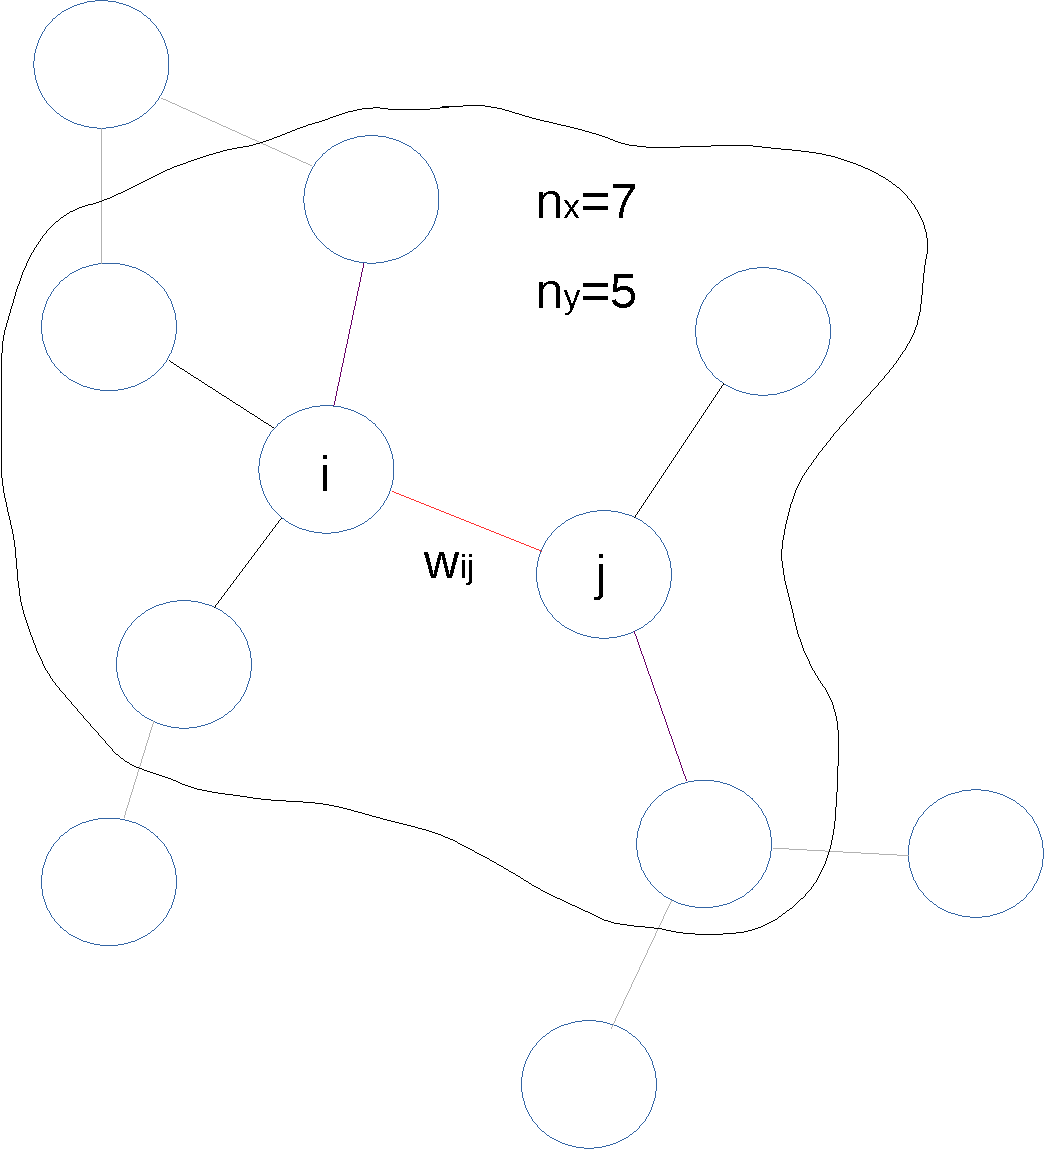
\includegraphics[width=0.8\textwidth]{vecindario_local.pdf}\\
    \bigskip
    \Fontvi
	A modo de ejemplo, la red para tratamiento ``Frío'' consta de 1951 nodos y 18436 aristas.
\end{columns}
\end{frame}

\begin{frame}\frametitle{Caracterización de vecindades locales tratamiento ``Frío''} 
\begin{columns}[T]
	\column{0.5\textwidth}
    \centering
    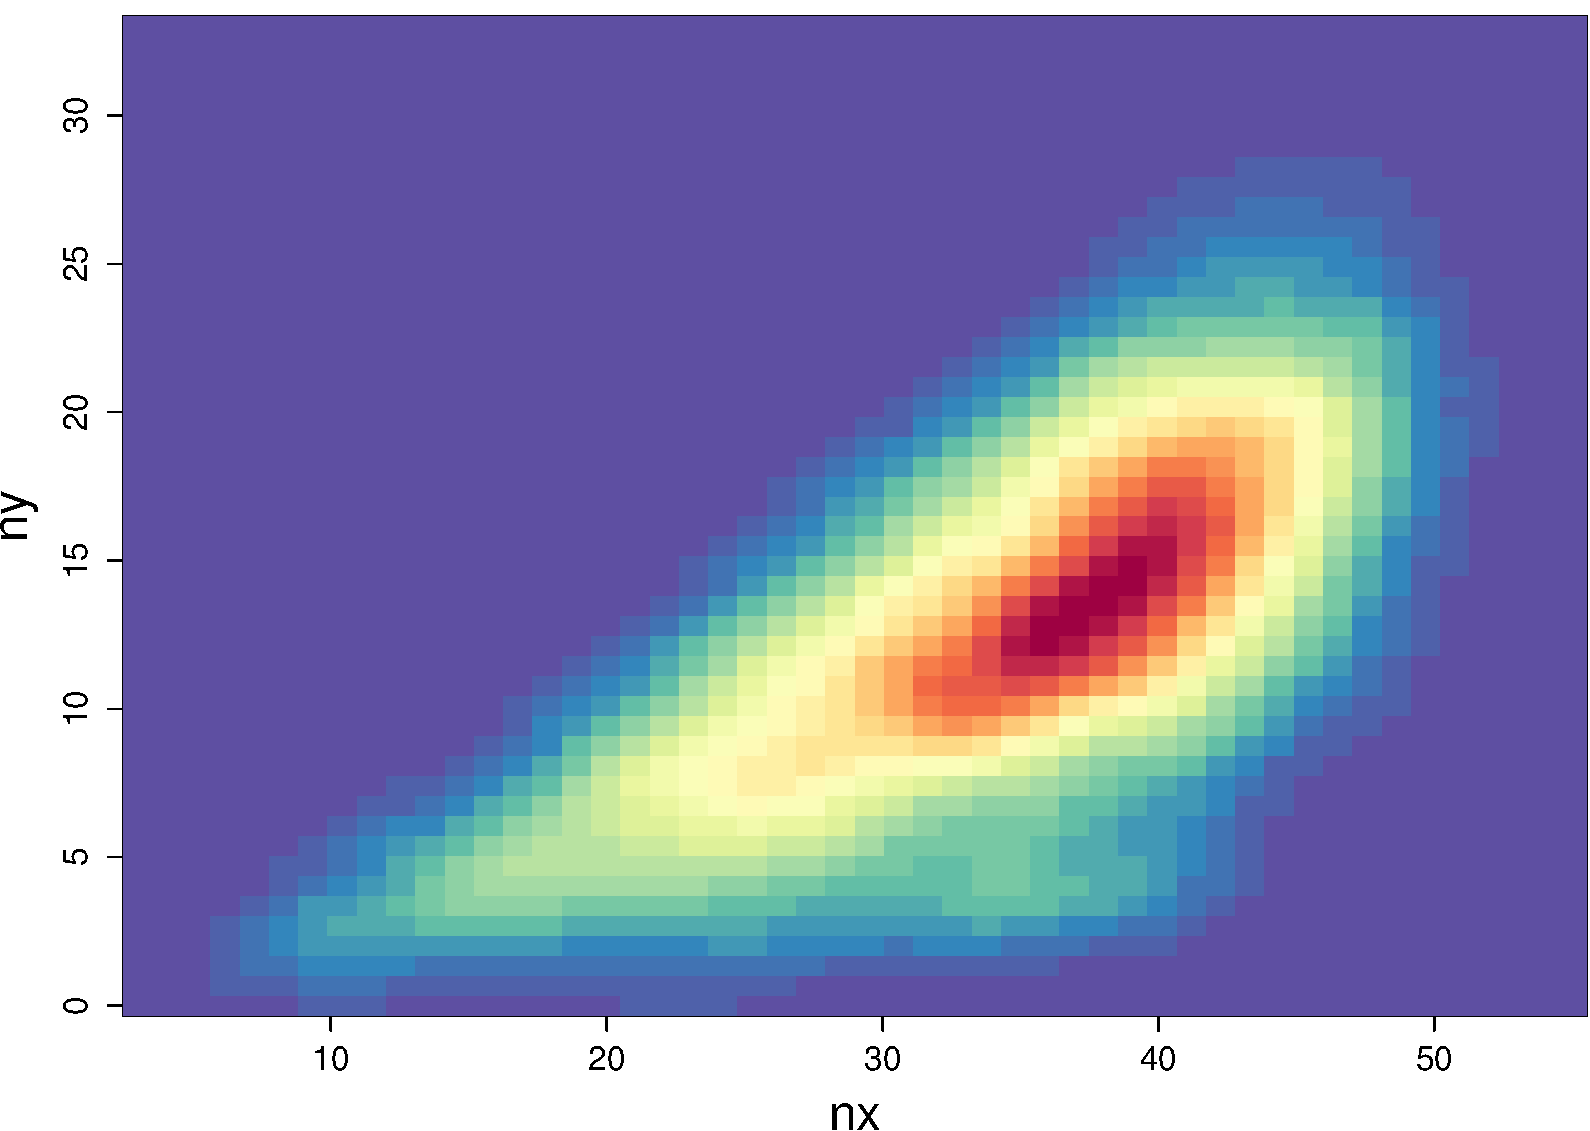
\includegraphics[width=0.90\textwidth]{nx_vs_ny.pdf}
    
    \centering
    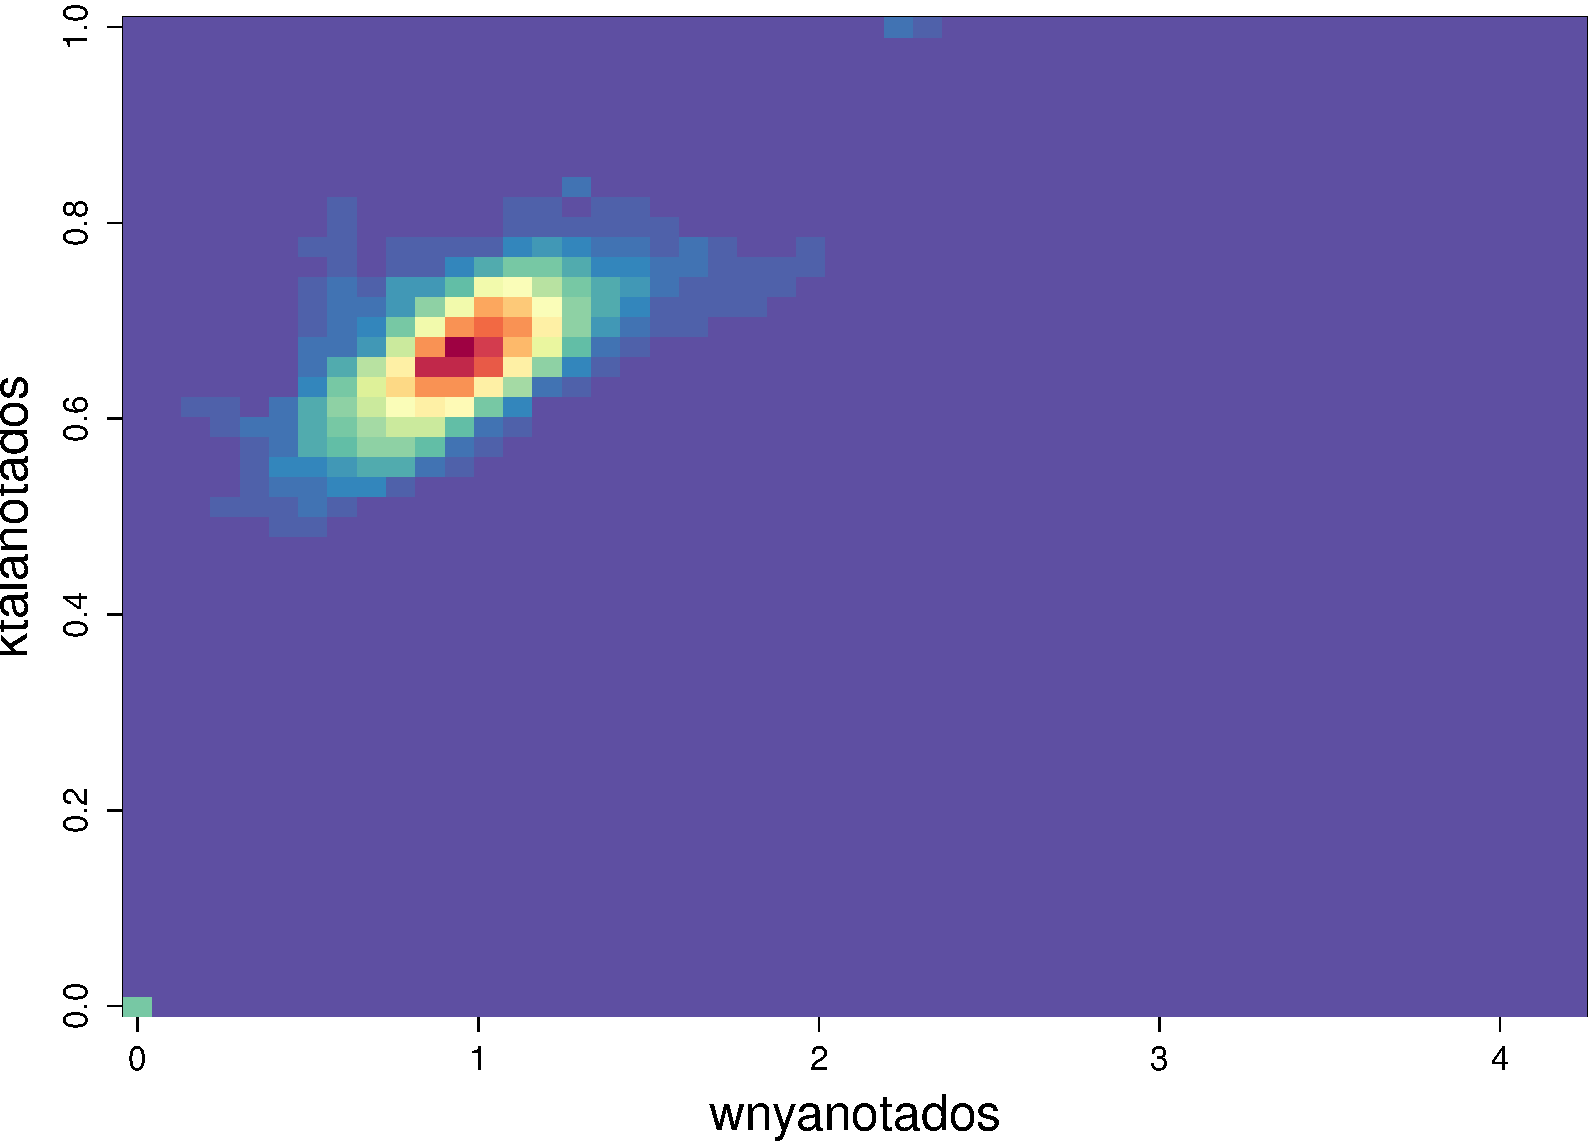
\includegraphics[width=0.90\textwidth]{lktaanotados_vs_wnyanotados.pdf}
	\column{0.5\textwidth}    
    \centering
    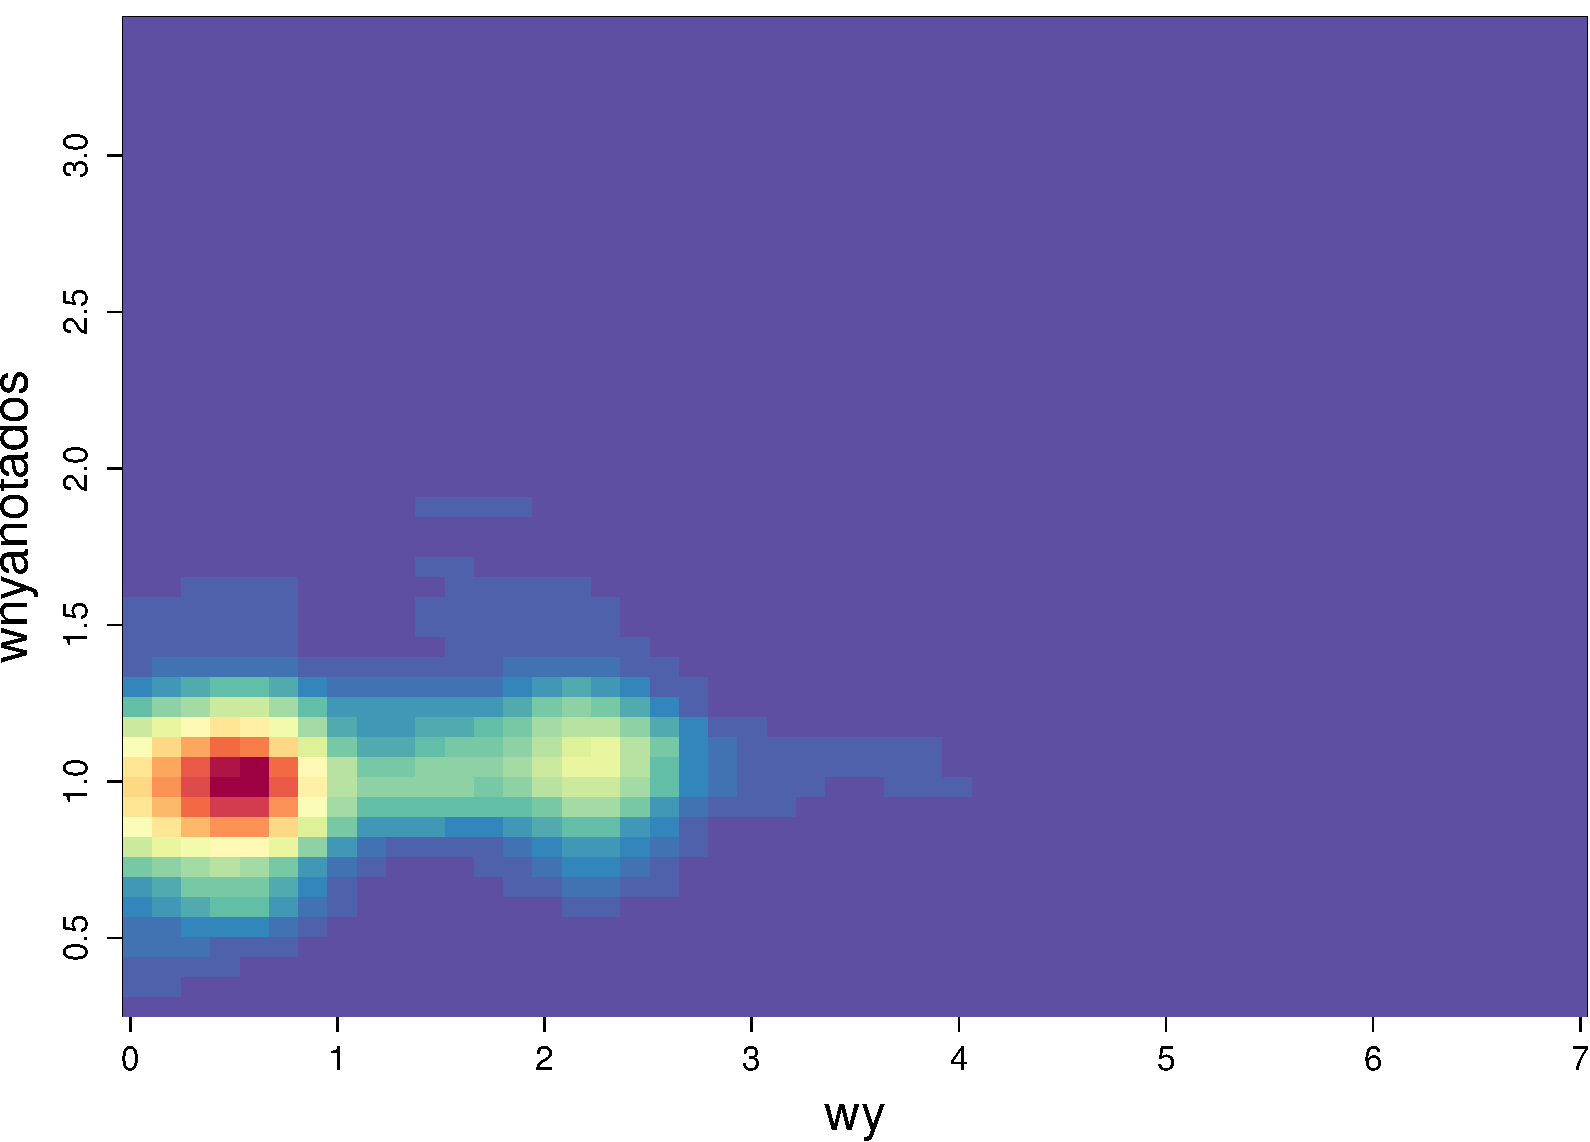
\includegraphics[width=0.90\textwidth]{wy_vs_wynanotados.pdf}
    
    \centering    
    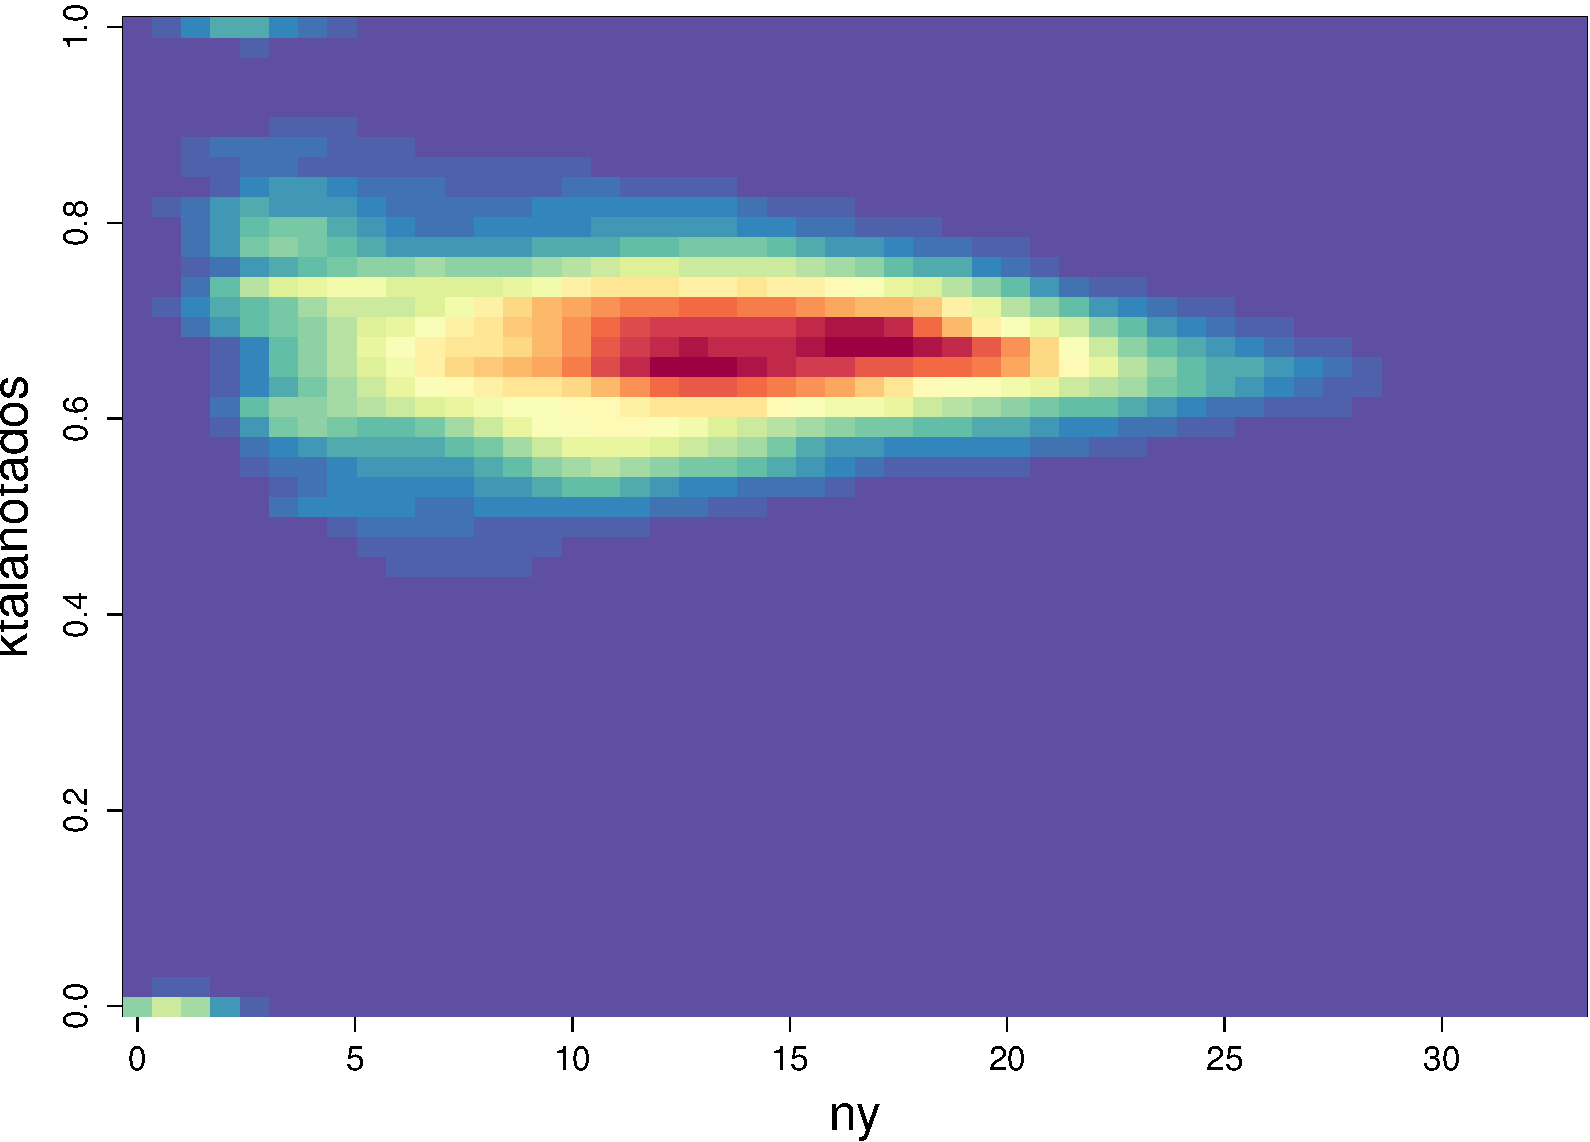
\includegraphics[width=0.90\textwidth]{lktaanotados_vs_nyanotados.pdf}
\end{columns}
\end{frame}

\subsubsection*{Métrica mixta}
\begin{frame}\frametitle{Métrica mixta} 
Dada una arista, el peso de una arista y el promedio de pesos, tenemos una manera de cuantificar si una vecindad es o no biologicamente coherente.\\
\bigskip
Vamos a usar esto para encontrar grupos transcripcionales teniendo en cuenta las coherencias biológicas locales modificando los pesos:
\bigskip
\begin{equation}
	w_{ij} = simcor_{ij}^{\beta*stress_{ij}}
\end{equation}
Donde:
\begin{equation}
	stress_{ij} = \frac{KTA_{fondo}}{KTAl_{ij}}
\end{equation}
\bigskip
Típicamente el $stress$ oscila entre $0.8$ y $1.2$.\\
\bigskip
$\beta$ es un parámetro que va a acentuar las heterogeneidades para poder detectar subgrupos.
\end{frame}

\subsubsection*{Métrica mixta y métodos heurísticos}
\begin{frame}\frametitle{Métrica mixta y métodos heurísticos} 
\bigskip
\centering
Buscamos subestructura en los grupos a partir de la métrica mixta\\
\vspace{10pt}
\begin{columns}
\column{\dimexpr\paperwidth-30pt}
\begin{columns}[T]
	\column{0.3\textwidth}
	Heurísticas con métrica mixta:
	\begin{itemize}
	\item lkta.dtc
	\item lkta.cnm
	\item lkta.infomap
	\end{itemize}
	Comparación con métrica transcripcional:
	\begin{itemize}
		\item InsideX
	\end{itemize}
	\column{0.7\textwidth}
	\vspace{10pt}
	\centering
	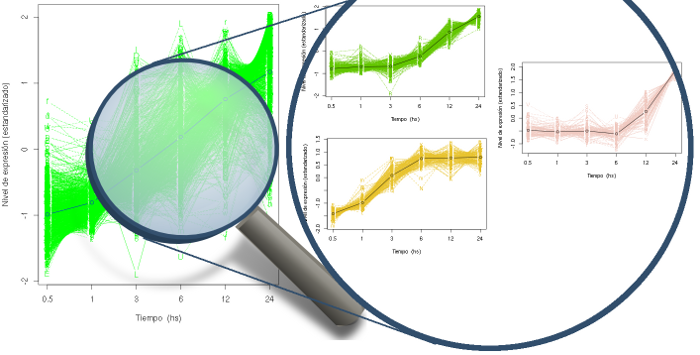
\includegraphics[width=1\textwidth]{lupa_chica.png}
\end{columns}
\end{columns}
\end{frame}

\begin{frame}\frametitle{Coherencia biológica medida con BHI - Ejemplo} 
\centering
Subestructura en grupo 2 de tratamiento ``Frío''\\
\begin{figure}
\centering
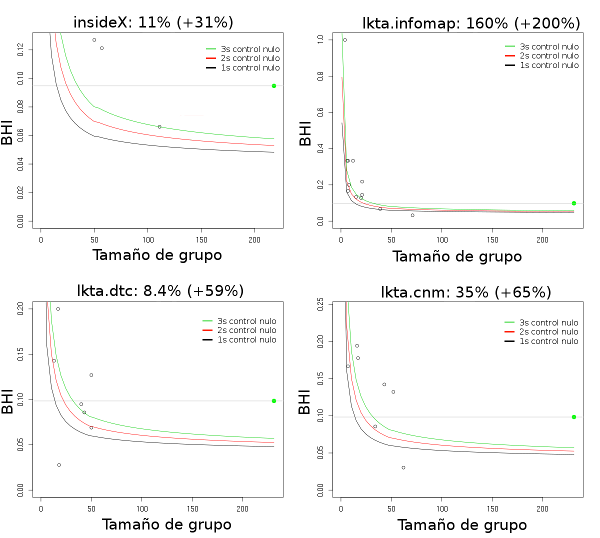
\includegraphics[width=0.7\textwidth]{metodos_mixtos_grupo_2_chico.png}
\end{figure}
\end{frame}

\begin{frame}\frametitle{Coherencia biológica medida con BHI} 
\centering
Caracterizamos los nuevos subgrupos hallados\\
\vspace{20pt}
\begin{figure}
\centering
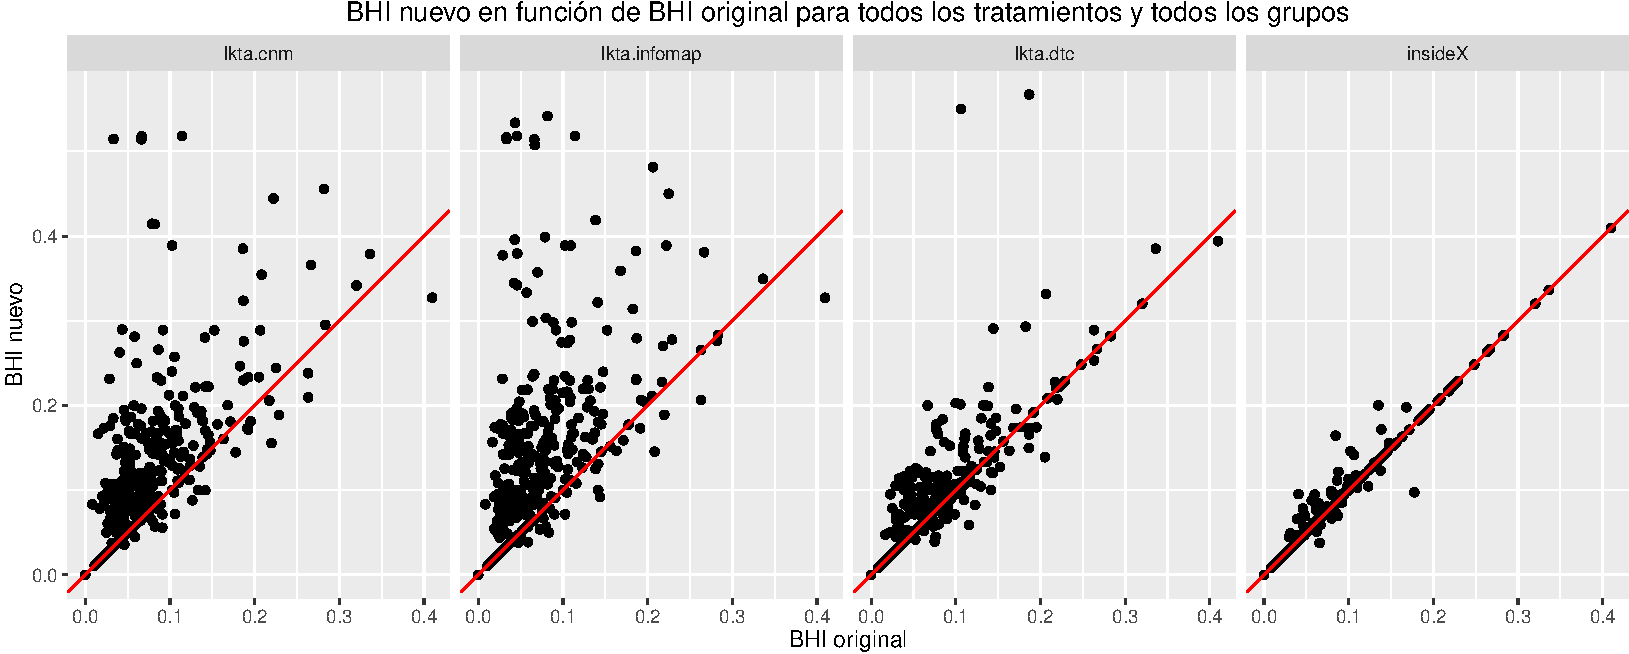
\includegraphics[width=1\textwidth]{bhi_nuevo_vs_bhi_original.pdf}
\end{figure}
\end{frame}

\subsubsection*{Coherencia biológica a partir de sobrerepresentación (test de Fisher)}
\begin{frame}\frametitle{Coherencia biológica a partir de sobrerepresentación (test de Fisher)} 
\vspace{-30pt}
\begin{columns}
\column{\dimexpr\paperwidth-10pt}
\begin{figure}
\centering
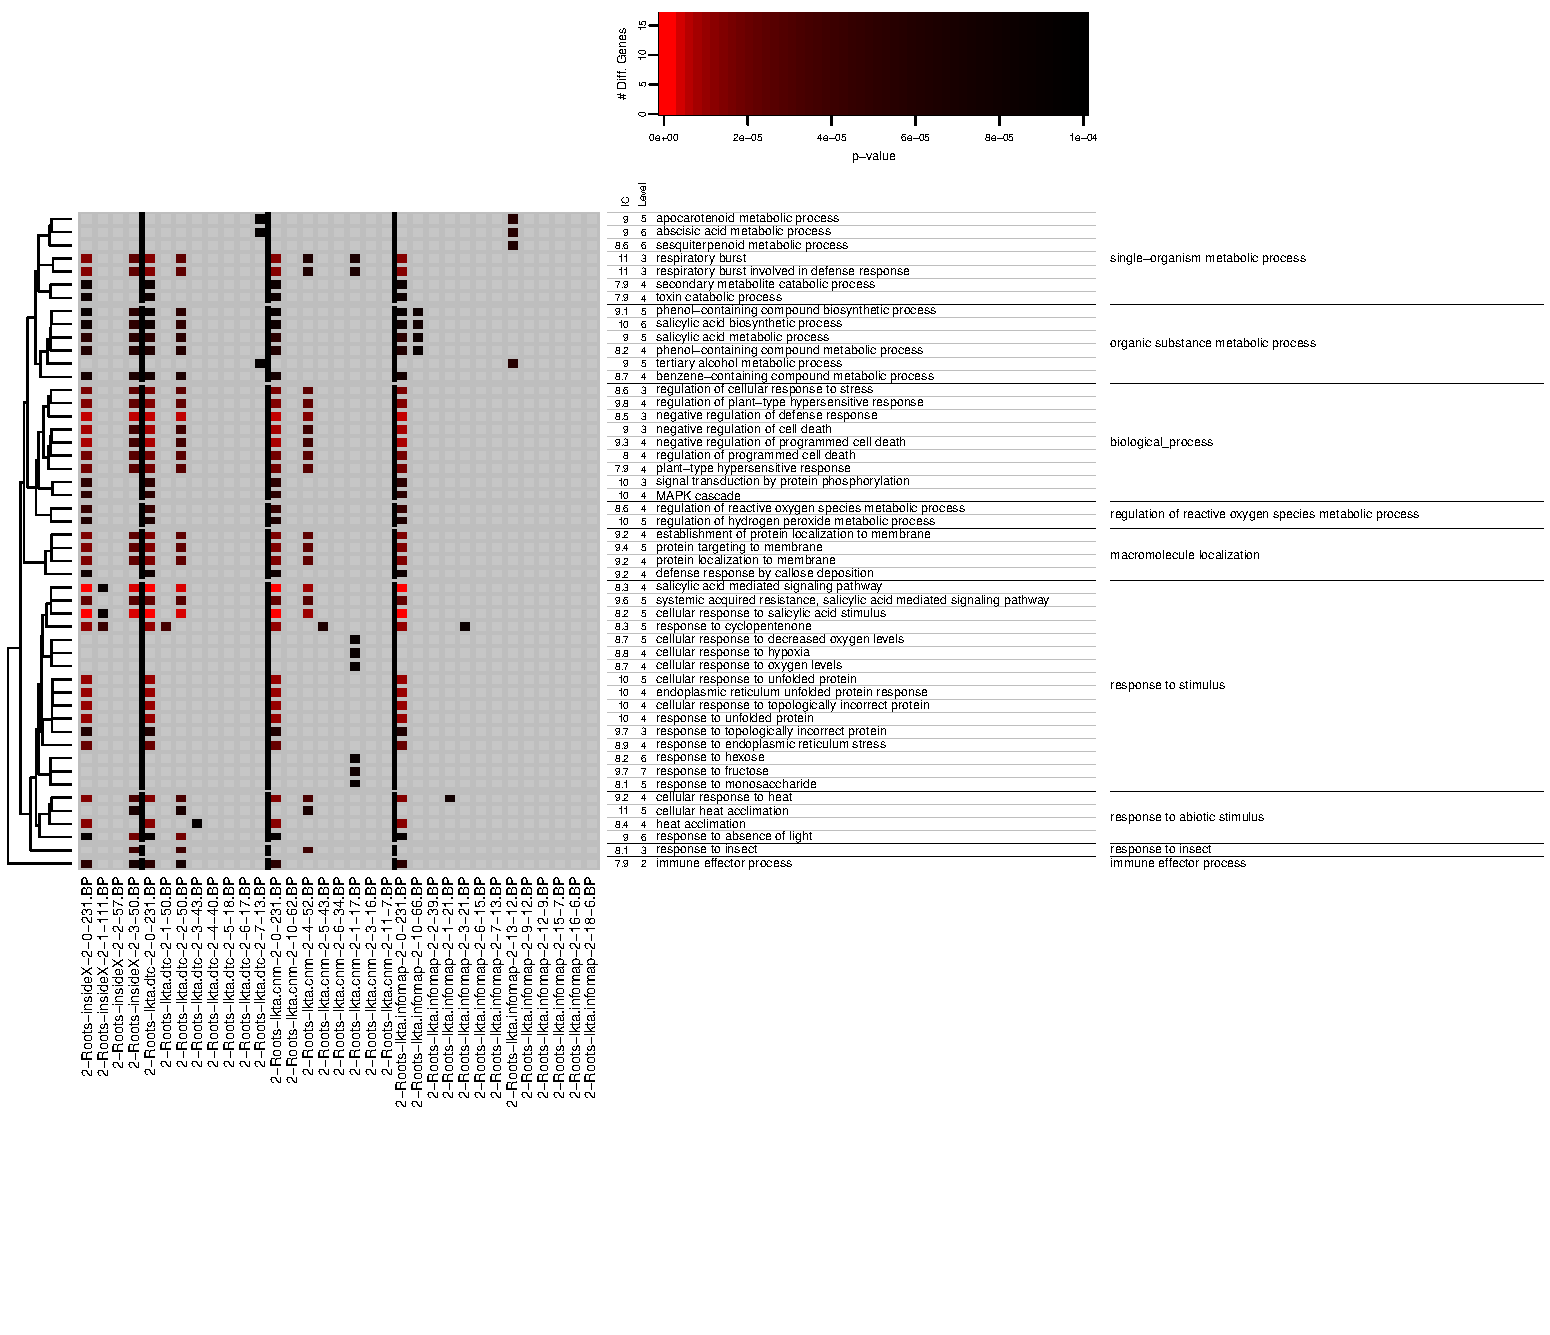
\includegraphics[width=0.95\textwidth]{fisher_grupo_2.pdf}
\end{figure}
\end{columns}
\end{frame}

\section{Conclusiones}
\begin{frame}\frametitle{Conclusiones}
\bigskip
\begin{itemize}
\item Diferentes técnicas de agrupamiento nos permitieron obtener grupos correlacionados en el espacio de expresión.
\item Cada método obtiene descripciones a diferente resolución.
\item Buscamos analizar estas descripciones en función de la interpretabilidad biológica.
\item Presentamos los observables BHI y KTA para cuantificar la coherencia entre los espacios y corroboramos que lo detectado en el espacio transcripcional es en general coherente con el conocimiento biológico.
\item Introdujimos una versión local de KTA que nos permitió definir una métrica mixta.
\item Presentamos heurísticas para identificar subestructuras transcripcionales con alta interpretabilidad y coherencia biológica.
\end{itemize}
\end{frame}

\begin{frame}\frametitle{Muchas gracias}
\huge
\centering
¡Muchas gracias por su atención!

\vspace{50pt}
¿Preguntas o comentarios?

\end{frame}

\begin{frame}\frametitle{Agradecimientos}
\begin{figure}
\centering
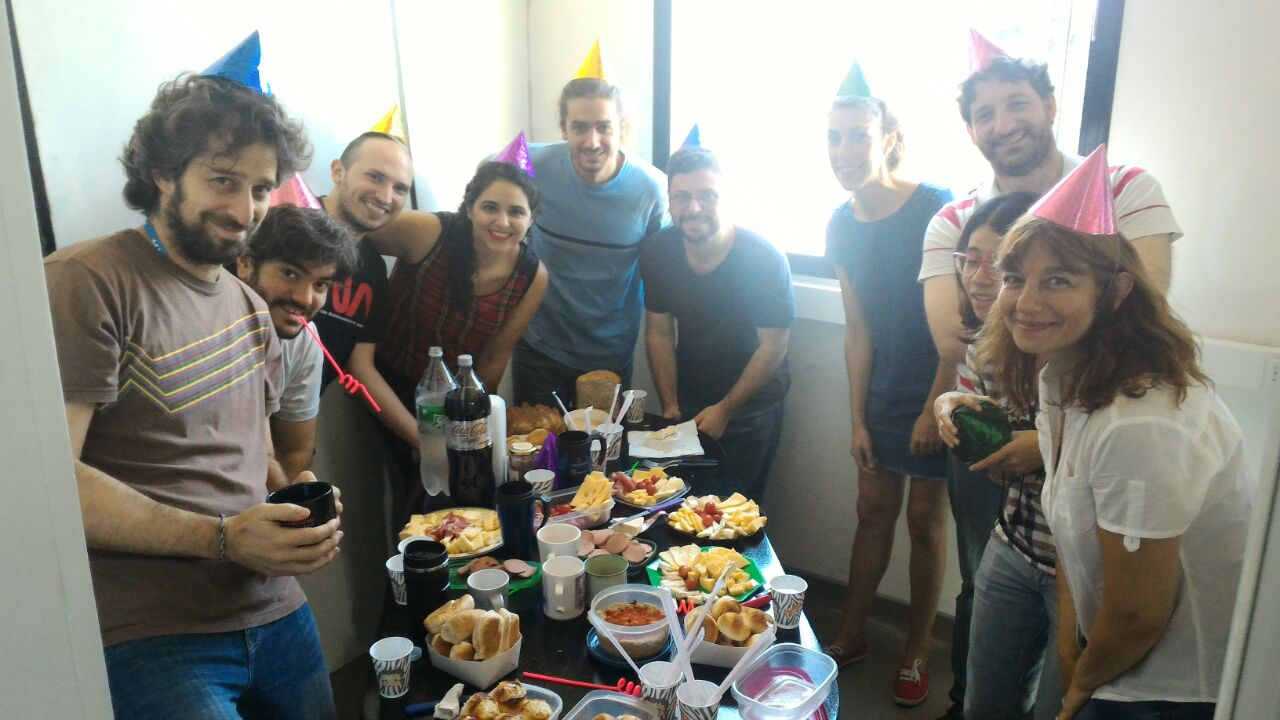
\includegraphics[width=1\textwidth]{grupo.jpeg}
\end{figure}
\end{frame}

\end{document}